% Options for packages loaded elsewhere
\PassOptionsToPackage{unicode}{hyperref}
\PassOptionsToPackage{hyphens}{url}
\PassOptionsToPackage{dvipsnames,svgnames,x11names}{xcolor}
%
\documentclass[
  letterpaper,
  DIV=11,
  numbers=noendperiod]{scrartcl}

\usepackage{amsmath,amssymb}
\usepackage{iftex}
\ifPDFTeX
  \usepackage[T1]{fontenc}
  \usepackage[utf8]{inputenc}
  \usepackage{textcomp} % provide euro and other symbols
\else % if luatex or xetex
  \usepackage{unicode-math}
  \defaultfontfeatures{Scale=MatchLowercase}
  \defaultfontfeatures[\rmfamily]{Ligatures=TeX,Scale=1}
\fi
\usepackage{lmodern}
\ifPDFTeX\else  
    % xetex/luatex font selection
\fi
% Use upquote if available, for straight quotes in verbatim environments
\IfFileExists{upquote.sty}{\usepackage{upquote}}{}
\IfFileExists{microtype.sty}{% use microtype if available
  \usepackage[]{microtype}
  \UseMicrotypeSet[protrusion]{basicmath} % disable protrusion for tt fonts
}{}
\makeatletter
\@ifundefined{KOMAClassName}{% if non-KOMA class
  \IfFileExists{parskip.sty}{%
    \usepackage{parskip}
  }{% else
    \setlength{\parindent}{0pt}
    \setlength{\parskip}{6pt plus 2pt minus 1pt}}
}{% if KOMA class
  \KOMAoptions{parskip=half}}
\makeatother
\usepackage{xcolor}
\setlength{\emergencystretch}{3em} % prevent overfull lines
\setcounter{secnumdepth}{5}
% Make \paragraph and \subparagraph free-standing
\ifx\paragraph\undefined\else
  \let\oldparagraph\paragraph
  \renewcommand{\paragraph}[1]{\oldparagraph{#1}\mbox{}}
\fi
\ifx\subparagraph\undefined\else
  \let\oldsubparagraph\subparagraph
  \renewcommand{\subparagraph}[1]{\oldsubparagraph{#1}\mbox{}}
\fi

\usepackage{color}
\usepackage{fancyvrb}
\newcommand{\VerbBar}{|}
\newcommand{\VERB}{\Verb[commandchars=\\\{\}]}
\DefineVerbatimEnvironment{Highlighting}{Verbatim}{commandchars=\\\{\}}
% Add ',fontsize=\small' for more characters per line
\usepackage{framed}
\definecolor{shadecolor}{RGB}{241,243,245}
\newenvironment{Shaded}{\begin{snugshade}}{\end{snugshade}}
\newcommand{\AlertTok}[1]{\textcolor[rgb]{0.68,0.00,0.00}{#1}}
\newcommand{\AnnotationTok}[1]{\textcolor[rgb]{0.37,0.37,0.37}{#1}}
\newcommand{\AttributeTok}[1]{\textcolor[rgb]{0.40,0.45,0.13}{#1}}
\newcommand{\BaseNTok}[1]{\textcolor[rgb]{0.68,0.00,0.00}{#1}}
\newcommand{\BuiltInTok}[1]{\textcolor[rgb]{0.00,0.23,0.31}{#1}}
\newcommand{\CharTok}[1]{\textcolor[rgb]{0.13,0.47,0.30}{#1}}
\newcommand{\CommentTok}[1]{\textcolor[rgb]{0.37,0.37,0.37}{#1}}
\newcommand{\CommentVarTok}[1]{\textcolor[rgb]{0.37,0.37,0.37}{\textit{#1}}}
\newcommand{\ConstantTok}[1]{\textcolor[rgb]{0.56,0.35,0.01}{#1}}
\newcommand{\ControlFlowTok}[1]{\textcolor[rgb]{0.00,0.23,0.31}{#1}}
\newcommand{\DataTypeTok}[1]{\textcolor[rgb]{0.68,0.00,0.00}{#1}}
\newcommand{\DecValTok}[1]{\textcolor[rgb]{0.68,0.00,0.00}{#1}}
\newcommand{\DocumentationTok}[1]{\textcolor[rgb]{0.37,0.37,0.37}{\textit{#1}}}
\newcommand{\ErrorTok}[1]{\textcolor[rgb]{0.68,0.00,0.00}{#1}}
\newcommand{\ExtensionTok}[1]{\textcolor[rgb]{0.00,0.23,0.31}{#1}}
\newcommand{\FloatTok}[1]{\textcolor[rgb]{0.68,0.00,0.00}{#1}}
\newcommand{\FunctionTok}[1]{\textcolor[rgb]{0.28,0.35,0.67}{#1}}
\newcommand{\ImportTok}[1]{\textcolor[rgb]{0.00,0.46,0.62}{#1}}
\newcommand{\InformationTok}[1]{\textcolor[rgb]{0.37,0.37,0.37}{#1}}
\newcommand{\KeywordTok}[1]{\textcolor[rgb]{0.00,0.23,0.31}{#1}}
\newcommand{\NormalTok}[1]{\textcolor[rgb]{0.00,0.23,0.31}{#1}}
\newcommand{\OperatorTok}[1]{\textcolor[rgb]{0.37,0.37,0.37}{#1}}
\newcommand{\OtherTok}[1]{\textcolor[rgb]{0.00,0.23,0.31}{#1}}
\newcommand{\PreprocessorTok}[1]{\textcolor[rgb]{0.68,0.00,0.00}{#1}}
\newcommand{\RegionMarkerTok}[1]{\textcolor[rgb]{0.00,0.23,0.31}{#1}}
\newcommand{\SpecialCharTok}[1]{\textcolor[rgb]{0.37,0.37,0.37}{#1}}
\newcommand{\SpecialStringTok}[1]{\textcolor[rgb]{0.13,0.47,0.30}{#1}}
\newcommand{\StringTok}[1]{\textcolor[rgb]{0.13,0.47,0.30}{#1}}
\newcommand{\VariableTok}[1]{\textcolor[rgb]{0.07,0.07,0.07}{#1}}
\newcommand{\VerbatimStringTok}[1]{\textcolor[rgb]{0.13,0.47,0.30}{#1}}
\newcommand{\WarningTok}[1]{\textcolor[rgb]{0.37,0.37,0.37}{\textit{#1}}}

\providecommand{\tightlist}{%
  \setlength{\itemsep}{0pt}\setlength{\parskip}{0pt}}\usepackage{longtable,booktabs,array}
\usepackage{calc} % for calculating minipage widths
% Correct order of tables after \paragraph or \subparagraph
\usepackage{etoolbox}
\makeatletter
\patchcmd\longtable{\par}{\if@noskipsec\mbox{}\fi\par}{}{}
\makeatother
% Allow footnotes in longtable head/foot
\IfFileExists{footnotehyper.sty}{\usepackage{footnotehyper}}{\usepackage{footnote}}
\makesavenoteenv{longtable}
\usepackage{graphicx}
\makeatletter
\def\maxwidth{\ifdim\Gin@nat@width>\linewidth\linewidth\else\Gin@nat@width\fi}
\def\maxheight{\ifdim\Gin@nat@height>\textheight\textheight\else\Gin@nat@height\fi}
\makeatother
% Scale images if necessary, so that they will not overflow the page
% margins by default, and it is still possible to overwrite the defaults
% using explicit options in \includegraphics[width, height, ...]{}
\setkeys{Gin}{width=\maxwidth,height=\maxheight,keepaspectratio}
% Set default figure placement to htbp
\makeatletter
\def\fps@figure{htbp}
\makeatother
% definitions for citeproc citations
\NewDocumentCommand\citeproctext{}{}
\NewDocumentCommand\citeproc{mm}{%
  \begingroup\def\citeproctext{#2}\cite{#1}\endgroup}
\makeatletter
 % allow citations to break across lines
 \let\@cite@ofmt\@firstofone
 % avoid brackets around text for \cite:
 \def\@biblabel#1{}
 \def\@cite#1#2{{#1\if@tempswa , #2\fi}}
\makeatother
\newlength{\cslhangindent}
\setlength{\cslhangindent}{1.5em}
\newlength{\csllabelwidth}
\setlength{\csllabelwidth}{3em}
\newenvironment{CSLReferences}[2] % #1 hanging-indent, #2 entry-spacing
 {\begin{list}{}{%
  \setlength{\itemindent}{0pt}
  \setlength{\leftmargin}{0pt}
  \setlength{\parsep}{0pt}
  % turn on hanging indent if param 1 is 1
  \ifodd #1
   \setlength{\leftmargin}{\cslhangindent}
   \setlength{\itemindent}{-1\cslhangindent}
  \fi
  % set entry spacing
  \setlength{\itemsep}{#2\baselineskip}}}
 {\end{list}}
\usepackage{calc}
\newcommand{\CSLBlock}[1]{\hfill\break\parbox[t]{\linewidth}{\strut\ignorespaces#1\strut}}
\newcommand{\CSLLeftMargin}[1]{\parbox[t]{\csllabelwidth}{\strut#1\strut}}
\newcommand{\CSLRightInline}[1]{\parbox[t]{\linewidth - \csllabelwidth}{\strut#1\strut}}
\newcommand{\CSLIndent}[1]{\hspace{\cslhangindent}#1}

% load packages
\usepackage{geometry}
\usepackage{xcolor}
\usepackage{eso-pic}
\usepackage{fancyhdr}
\usepackage{sectsty}
\usepackage{fontspec}
\usepackage{titlesec}

%% Set page size with a wider right margin
\geometry{a4paper, total={170mm,257mm}, left=20mm, top=20mm, bottom=20mm, right=50mm}

%% Let's define some colours
\definecolor{uniblue}{HTML}{003865}
\definecolor{burgundy}{HTML}{7D2239}
\definecolor{cobalt}{HTML}{005C8A}
\definecolor{lavender}{HTML}{5B4D94}
\definecolor{leaf}{HTML}{006630}
\definecolor{moss}{HTML}{385A4F}
\definecolor{pillarbox}{HTML}{B30C00}
\definecolor{rust}{HTML}{9A3A06}
\definecolor{sandstone}{HTML}{52473B}
\definecolor{skyblue}{HTML}{005398}
\definecolor{slate}{HTML}{4F5961}
\definecolor{thistle}{HTML}{951272}

%\definecolor{light}{HTML}{E6E6FA} % original from template - redefined below as uni blue at 10 percent:
\colorlet{light}{uniblue!10}
%\definecolor{highlight}{HTML}{800080} % original from template - redefined below as uni's skyblue:
\colorlet{highlight}{skyblue}
%\definecolor{dark}{HTML}{330033} % original from template - redefined below as uni blue at 100 percent:
\colorlet{dark}{uniblue}

%% Let's add the border on the right hand side 
\AddToShipoutPicture{% 
    \AtPageLowerLeft{% 
        \put(\LenToUnit{\dimexpr\paperwidth-3cm},0){% 
            \color{light}\rule{3cm}{\LenToUnit\paperheight}%
          }%
     }%
     % logo
    \AtPageLowerLeft{% start the bar at the bottom right of the page
        \put(\LenToUnit{\dimexpr\paperwidth-2.25cm},27.2cm){% move it to the top right
            \color{light}
\includegraphics[width=2.25cm]{_extensions/nrennie/PrettyPDF/uni_logo_boxed.jpg}
          }%
     }%
}

%% Style the page number
\fancypagestyle{mystyle}{
  \fancyhf{}
  \renewcommand\headrulewidth{0pt}
  \fancyfoot[R]{\thepage}
  \fancyfootoffset{3.5cm}
}
\setlength{\footskip}{20pt}

%% style the chapter/section fonts
\chapterfont{\color{uniblue}\fontsize{20}{16.8}\selectfont}
\sectionfont{\color{uniblue}\fontsize{20}{16.8}\selectfont}
\subsectionfont{\color{skyblue}\fontsize{14}{16.8}\selectfont}
\titleformat{\subsection}
  {\color{uniblue!90}\sffamily\Large\bfseries}{\thesubsection}{1em}{}[{\titlerule[0.8pt]}]
\subsubsectionfont{\color{cobalt}}

\renewcommand\thesection{\color{slate}\arabic{section}}
  
% left align title
\makeatletter
\renewcommand{\maketitle}{\bgroup\setlength{\parindent}{0pt}
\begin{flushleft}
  {\color{uniblue}\sffamily\huge\textbf{\@title}} \vspace{0.3cm} \newline
  {\Large {\@subtitle}} \newline
  \@author
\end{flushleft}\egroup
}
\makeatother

%% Use some custom fonts
\setsansfont{Ubuntu}[
    Path=_extensions/nrennie/PrettyPDF/Ubuntu/,
    Scale=0.9,
    Extension = .ttf,
    UprightFont=*-Regular,
    BoldFont=*-Bold,
    ItalicFont=*-Italic,
    ]

\setmainfont{Ubuntu}[
    Path=_extensions/nrennie/PrettyPDF/Ubuntu/,
    Scale=0.9,
    Extension = .ttf,
    UprightFont=*-Regular,
    BoldFont=*-Bold,
    ItalicFont=*-Italic,
    ]
\usepackage{booktabs}
\usepackage{longtable}
\usepackage{array}
\usepackage{multirow}
\usepackage{wrapfig}
\usepackage{float}
\usepackage{colortbl}
\usepackage{pdflscape}
\usepackage{tabu}
\usepackage{threeparttable}
\usepackage{threeparttablex}
\usepackage[normalem]{ulem}
\usepackage{makecell}
\usepackage{xcolor}
\KOMAoption{captions}{tableheading}
\makeatletter
\@ifpackageloaded{tcolorbox}{}{\usepackage[skins,breakable]{tcolorbox}}
\@ifpackageloaded{fontawesome5}{}{\usepackage{fontawesome5}}
\definecolor{quarto-callout-color}{HTML}{909090}
\definecolor{quarto-callout-note-color}{HTML}{0758E5}
\definecolor{quarto-callout-important-color}{HTML}{CC1914}
\definecolor{quarto-callout-warning-color}{HTML}{EB9113}
\definecolor{quarto-callout-tip-color}{HTML}{00A047}
\definecolor{quarto-callout-caution-color}{HTML}{FC5300}
\definecolor{quarto-callout-color-frame}{HTML}{acacac}
\definecolor{quarto-callout-note-color-frame}{HTML}{4582ec}
\definecolor{quarto-callout-important-color-frame}{HTML}{d9534f}
\definecolor{quarto-callout-warning-color-frame}{HTML}{f0ad4e}
\definecolor{quarto-callout-tip-color-frame}{HTML}{02b875}
\definecolor{quarto-callout-caution-color-frame}{HTML}{fd7e14}
\makeatother
\makeatletter
\@ifpackageloaded{caption}{}{\usepackage{caption}}
\AtBeginDocument{%
\ifdefined\contentsname
  \renewcommand*\contentsname{Table of contents}
\else
  \newcommand\contentsname{Table of contents}
\fi
\ifdefined\listfigurename
  \renewcommand*\listfigurename{List of Figures}
\else
  \newcommand\listfigurename{List of Figures}
\fi
\ifdefined\listtablename
  \renewcommand*\listtablename{List of Tables}
\else
  \newcommand\listtablename{List of Tables}
\fi
\ifdefined\figurename
  \renewcommand*\figurename{Figure}
\else
  \newcommand\figurename{Figure}
\fi
\ifdefined\tablename
  \renewcommand*\tablename{Table}
\else
  \newcommand\tablename{Table}
\fi
}
\@ifpackageloaded{float}{}{\usepackage{float}}
\floatstyle{ruled}
\@ifundefined{c@chapter}{\newfloat{codelisting}{h}{lop}}{\newfloat{codelisting}{h}{lop}[chapter]}
\floatname{codelisting}{Listing}
\newcommand*\listoflistings{\listof{codelisting}{List of Listings}}
\makeatother
\makeatletter
\makeatother
\makeatletter
\@ifpackageloaded{caption}{}{\usepackage{caption}}
\@ifpackageloaded{subcaption}{}{\usepackage{subcaption}}
\makeatother
\makeatletter
\@ifpackageloaded{tcolorbox}{}{\usepackage[skins,breakable]{tcolorbox}}
\makeatother
\makeatletter
\@ifundefined{shadecolor}{\definecolor{shadecolor}{rgb}{.97, .97, .97}}{}
\makeatother
\makeatletter
\@ifundefined{codebgcolor}{\definecolor{codebgcolor}{named}{light}}{}
\makeatother
\makeatletter
\ifdefined\Shaded\renewenvironment{Shaded}{\begin{tcolorbox}[colback={codebgcolor}, enhanced, boxrule=0pt, breakable, frame hidden, sharp corners]}{\end{tcolorbox}}\fi
\makeatother
\ifLuaTeX
  \usepackage{selnolig}  % disable illegal ligatures
\fi
\usepackage{bookmark}

\IfFileExists{xurl.sty}{\usepackage{xurl}}{} % add URL line breaks if available
\urlstyle{same} % disable monospaced font for URLs
\hypersetup{
  pdftitle={Generalised Linear Models part 1},
  colorlinks=true,
  linkcolor={highlight},
  filecolor={Maroon},
  citecolor={Blue},
  urlcolor={highlight},
  pdfcreator={LaTeX via pandoc}}

\title{Generalised Linear Models part 1}
\author{}
\date{}

\begin{document}
\maketitle

\pagestyle{mystyle}

\section{Introduction}\label{introduction}

In previous weeks we looked at modelling data using linear regression
models were we had:

\begin{itemize}
\tightlist
\item
  a \textbf{continuous response variable} \(y\) and
\item
  one or more \textbf{explanatory variables} \(x_1, x_2,\ldots, x_p\),
  which were \textbf{numerical}/\textbf{categorical} variables.
\end{itemize}

Recall that for data \((y_i, x_i), ~ i = 1,\ldots, n\), where \(y\) is a
continuous response variable, we can write a simple linear regression
model as follows:

\[y_i = \alpha + \beta x_i + \epsilon_i, ~~~~ \epsilon_i \sim N(0, \sigma^2),\]
where

\begin{itemize}
\tightlist
\item
  \(y_i\) is the \(i^{th}\) observation of the continuous response
  variable;
\item
  \(\alpha\) is the \textbf{intercept} of the regression line;
\item
  \(\beta\) is the \textbf{slope} of the regression line;
\item
  \(x_i\) is the \(i^{th}\) observation of the explanatory variable; and
\item
  \(\epsilon_i\) is the \(i^{th}\) random component.
\end{itemize}

Thus, the full probability model for \(y_i\) given \(x_i\)
(\(y_i | x_i\)) can be written as

\[y_i | x_i \sim N(\alpha + \beta x_i, \sigma^2),\]

where the mean \(\alpha + \beta x_i\) is given by the deterministic part
of the model and the variance \(\sigma^2\) by the random part. Hence we
make the assumption that the outcomes \(y_i\) are normally distributed
with mean \(\alpha + \beta x_i\) and variance \(\sigma^2\). However,
what if our response variable \(y\) is not a continuous random variable?

\subsection{Generalised linear models}\label{generalised-linear-models}

The main objective this week is to introduce \textbf{Generalised Linear
Models (GLMs)}, which extend the linear model framework to response
variables that don't follow the normal distribution. GLMs can be used to
model non-normal continuous response variables, but they are most
frequently used to model binary, categorical or count data. The
generalised linear model can be written as:

\vspace{-0.5cm}

\begin{align}
y_i &\sim f(g(\boldsymbol{\mu}_i)) \nonumber \\
\boldsymbol{\mu}_i &= \mathbf{x}_i^\top \boldsymbol{\beta}, \nonumber
\end{align}

where the response \(y_i\) is predicted through the linear combination
\(\boldsymbol{\mu}_i\) of explanatory variables by the link function
\(g(\cdot)\), assuming some distribution \(f(\cdot)\) for \(y_i\), and
\(\mathbf{x}_i^\top\) is the \(i^{th}\) row of the design matrix
\(\boldsymbol{X}\). For example, the simple linear regression model
above for a continuous response variable has the normal distribution
distribution as \(f(\cdot)\), with corresponding link function equal to
the Identity function, that is,
\(g(\boldsymbol{\mu}_i) = \boldsymbol{\mu}_i\).

This week we will learn how to model outcomes of interest that take one
of two categorical values (e.g.~yes/no, success/failure, alive/dead),
i.e.

\begin{itemize}
\tightlist
\item
  \textbf{binary}, taking the value 1 (say success, with probability
  \(p_i\)) or 0 (failure, with probability \(1-p_i\)) or
\end{itemize}

In this case, the distribution of \(y_i\) is assumed to be binomial
Bin\((1,p_i)\). Hence, a binary response variable \(y_i\) has a binomial
distribution with corresponding link function \(g(\cdot)\) , e.g.~the
\textbf{logit link} function, that is

\[g(p_i) = \log \left(\frac{p_i}{1 - p_i} \right),\]

which is also referred to as the \textbf{log-odds} (since
\(p_i ~ / ~ 1-p_i\) is an odds ratio). Why is such a transformation
required when looking at a binary response variable? Well here we are
interested in modelling the probability of success \(p_i\), and as we
know probabilities must be between 0 and 1
\(\left(p_i \in [0, 1]\right)\). So if we want to model the probability
of success using a linear model we need to ensure that the probabilities
obtained are between 0 and 1. However, if we just use the identity link
function, such that

\[p_i = \mathbf{x}_i^\top \boldsymbol{\beta},\] we would need to ensure
that in some way \(\mathbf{x}_i^\top \boldsymbol{\beta} \in [0, 1]\),
that is, the linear combination of the explanatory variables and their
corresponding regression coefficients was between 0 and 1. Hence some
restrictions of some sort would need to be put in place to ensure this
was the case. However, if we use the logit link function, such that

\[\log \left(\frac{p_i}{1 - p_i} \right) = \mathbf{x}_i^\top \boldsymbol{\beta},\]

no restrictions need to be in place on our estimates of the parameter
vector \(\boldsymbol{\beta}\), since the inverse of the logit link
function will always gives us valid probabilities since

\[p_i = \frac{\exp\left(\mathbf{x}_i^\top \boldsymbol{\beta}\right)}{1 + \exp\left(\mathbf{x}_i^\top \boldsymbol{\beta}\right)} ~~~ \in [0, 1].\]

This linear regression model with a binary response variable and logit
link function is referred to as \textbf{logistic regression}. As such,
when it comes to looking at binary response variables we shall be
looking at odds ratios and probabilities of success/failure. The table
below is a reminder of the distribution and link function used for the
normal model we have previously looked at as well as the logistic
regression model we shall be examining for the rest of this week.

\begin{longtable}[]{@{}
  >{\centering\arraybackslash}p{(\columnwidth - 6\tabcolsep) * \real{0.2222}}
  >{\centering\arraybackslash}p{(\columnwidth - 6\tabcolsep) * \real{0.2222}}
  >{\centering\arraybackslash}p{(\columnwidth - 6\tabcolsep) * \real{0.3333}}
  >{\centering\arraybackslash}p{(\columnwidth - 6\tabcolsep) * \real{0.2222}}@{}}
\toprule\noalign{}
\begin{minipage}[b]{\linewidth}\centering
\textbf{Model}
\end{minipage} & \begin{minipage}[b]{\linewidth}\centering
\textbf{Random component}
\end{minipage} & \begin{minipage}[b]{\linewidth}\centering
\textbf{Systematic component}
\end{minipage} & \begin{minipage}[b]{\linewidth}\centering
\textbf{Link function}
\end{minipage} \\
\midrule\noalign{}
\endhead
\bottomrule\noalign{}
\endlastfoot
Normal & \(y_i\overset{\text{indep}}\sim \text{N}(\mu_i,\sigma^2),\) &
\(\boldsymbol{x}_i^\top\boldsymbol{\beta} =\beta_0 + \beta_1x_i + \beta_2x_i + \ldots\)
& \(g(\mu_i)=\mu_i\) \\
Logistic & \(y_i\overset{\text{indep}}\sim \text{Bin}(1,p_i),\) &
\(\boldsymbol{x}_i^\top\boldsymbol{\beta} =\beta_0+ \beta_1x_i + \beta_2x_i + \ldots\)
& \(g(\mu_i) = \log \left( \frac{p_i}{1-p_i} \right)\) \\
\end{longtable}

\subsection*{Required R packages}\label{required-r-packages}
\addcontentsline{toc}{subsection}{Required R packages}

Before we proceed, load all the packages needed for this week:

\begin{Shaded}
\begin{Highlighting}[]
\FunctionTok{library}\NormalTok{(tidyverse)}
\FunctionTok{library}\NormalTok{(ggplot2)}
\FunctionTok{library}\NormalTok{(sjPlot)}
\FunctionTok{library}\NormalTok{(broom)}
\FunctionTok{library}\NormalTok{(performance)}
\FunctionTok{library}\NormalTok{(yardstick)  }\CommentTok{\# model validation}
\end{Highlighting}
\end{Shaded}

\section{Logistic regression with one numerical explanatory
variable}\label{logistic-regression-with-one-numerical-explanatory-variable}

Here we shall begin by fitting a logistic regression model with one
numerical explanatory variable. Let's return to the \texttt{evals} data
from the \texttt{moderndive} package that we examined in previous weeks.

\subsection{Teaching evaluation
scores}\label{teaching-evaluation-scores}

Student feedback in higher education is extremely important when it
comes to the evaluation of teaching techniques, materials, and
improvements in teaching methods and technologies. However, there have
been studies into potential bias factors when feedback is provided, such
as the physical appearance of the teacher; see
\href{https://www.journals.elsevier.com/economics-of-education-review/}{Economics
of Education Review} for details. Here, we shall look at a study from
student evaluations of \(n=463\) professors from The University of Texas
at Austin.

Previously, we looked at \textbf{teaching score} as our continuous
response variable and \textbf{beauty score} as our explanatory variable.
Now we shall consider \textbf{gender} as our response variable, and
hence shall have a binary response variable (female/male). We will
examine if there is any difference in \textbf{gender} by \textbf{age} of
the teaching instructors within the \texttt{evals} data set.

The data can be downloaded below:

You can download today's session R script below:

First, let's start by selecting the variables of interest from the
\texttt{evals} data set:

\begin{Shaded}
\begin{Highlighting}[]
\NormalTok{evals }\OtherTok{\textless{}{-}} \FunctionTok{read.csv}\NormalTok{(}\StringTok{"evals.csv"}\NormalTok{,}\AttributeTok{stringsAsFactors =}\NormalTok{ T)}
\NormalTok{evals.gender }\OtherTok{\textless{}{-}}\NormalTok{ evals }\SpecialCharTok{\%\textgreater{}\%}
                  \FunctionTok{select}\NormalTok{(gender, age)}
\end{Highlighting}
\end{Shaded}

Now, let's look at a boxplot of \texttt{age} by \texttt{gender} to get
an initial impression of the data:

\section{R plot}

\begin{figure}[H]

{\centering 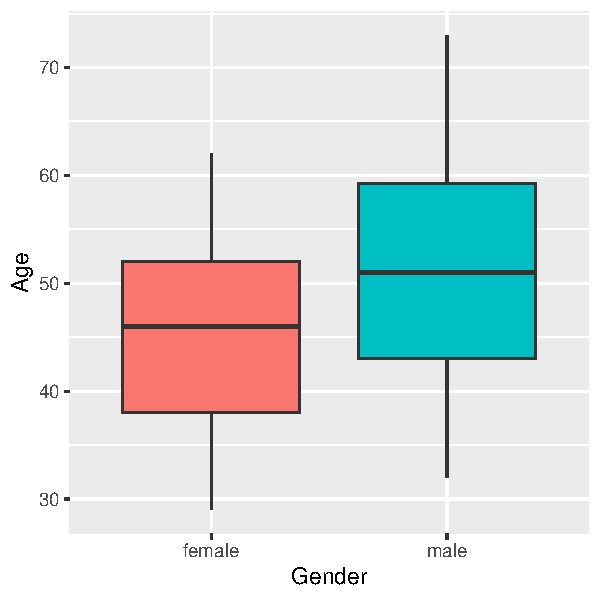
\includegraphics{index_files/figure-pdf/unnamed-chunk-4-1.pdf}

}

\caption{Teaching instructor age by gender.}

\end{figure}%

\section{R code}

\begin{Shaded}
\begin{Highlighting}[]
\FunctionTok{ggplot}\NormalTok{(}\AttributeTok{data =}\NormalTok{ evals.gender,}
       \FunctionTok{aes}\NormalTok{(}\AttributeTok{x =}\NormalTok{ gender, }\AttributeTok{y =}\NormalTok{ age, }\AttributeTok{fill =}\NormalTok{ gender)) }\SpecialCharTok{+}
  \FunctionTok{geom\_boxplot}\NormalTok{() }\SpecialCharTok{+}
  \FunctionTok{labs}\NormalTok{(}\AttributeTok{x =} \StringTok{"Gender"}\NormalTok{, }\AttributeTok{y =} \StringTok{"Age"}\NormalTok{) }\SpecialCharTok{+}
  \FunctionTok{theme}\NormalTok{(}\AttributeTok{legend.position =} \StringTok{"none"}\NormalTok{)}
\end{Highlighting}
\end{Shaded}

Here we can see that the age of male teaching instructors tends to be
higher than that of their female counterparts. Now, let's fit a logistic
regression model to see whether age is a significant predictor of the
odds of a teaching instructor being male or female.

\subsection{Log-odds}\label{log-odds}

To fit a logistic regression model we will use the generalised linear
model function \texttt{glm} and set the argument
\texttt{family\ =\ binomial}. The logistic regression model with
\textbf{gender} as the response and \textbf{age} as the explanatory
variable is given by:

\[
\begin{aligned}
\text{Gender}_i \sim \mathrm{Bernoulli}(p_i) \\
\log\left(\frac{p_i}{1-p_i}\right) = \alpha_0 +\beta_1 \times \text{Age}_i,
\end{aligned}
\]

and can be fitted in\texttt{R} as follows:

\begin{Shaded}
\begin{Highlighting}[]
\NormalTok{model }\OtherTok{\textless{}{-}} \FunctionTok{glm}\NormalTok{(gender }\SpecialCharTok{\textasciitilde{}}\NormalTok{ age, }\AttributeTok{data =}\NormalTok{ evals.gender,}\AttributeTok{family =}\NormalTok{ binomial)}
\end{Highlighting}
\end{Shaded}

This model uses the \textbf{logit link} function by default.

\begin{tcolorbox}[enhanced jigsaw, colframe=quarto-callout-note-color-frame, toprule=.15mm, toptitle=1mm, opacitybacktitle=0.6, breakable, colback=white, opacityback=0, title=\textcolor{quarto-callout-note-color}{\faInfo}\hspace{0.5em}{Note}, rightrule=.15mm, bottomrule=.15mm, coltitle=black, colbacktitle=quarto-callout-note-color!10!white, leftrule=.75mm, left=2mm, arc=.35mm, bottomtitle=1mm, titlerule=0mm]

To use a non-default or \texttt{link}, pass in as an argument to
\texttt{binomial()}. For example if we wanted to use the probit link
function we could specify the following argument:

\begin{Shaded}
\begin{Highlighting}[]
\FunctionTok{glm}\NormalTok{(gender }\SpecialCharTok{\textasciitilde{}}\NormalTok{ age,}
    \AttributeTok{data =}\NormalTok{ evals.gender,}
    \AttributeTok{family =} \FunctionTok{binomial}\NormalTok{(}\AttributeTok{link =} \StringTok{"probit"}\NormalTok{))}
\end{Highlighting}
\end{Shaded}

\end{tcolorbox}

Now, let's take a look at the summary produced from our logistic
regression model using the \texttt{tab\_model} function from the
\texttt{sjPlot} library by setting \texttt{transform\ =\ NULL} (this
will tell R to show the coefficients on the log-odds scale)

\begin{Shaded}
\begin{Highlighting}[]
\NormalTok{model }\SpecialCharTok{\%\textgreater{}\%} \FunctionTok{tab\_model}\NormalTok{(}\AttributeTok{show.ci =}\NormalTok{ F,}\AttributeTok{transform =} \ConstantTok{NULL}\NormalTok{)}
\end{Highlighting}
\end{Shaded}

\begin{longtable}[]{@{}ccc@{}}
\toprule\noalign{}
\endhead
\bottomrule\noalign{}
\endlastfoot
~ & \multicolumn{2}{c@{}}{%
gender} \\
Predictors & Log-Odds & p \\
(Intercept) & -2.70 & \textbf{\textless0.001} \\
age & 0.06 & \textbf{\textless0.001} \\
Observations & \multicolumn{2}{l@{}}{%
463} \\
R\textsuperscript{2} Tjur & \multicolumn{2}{l@{}}{%
0.079} \\
\end{longtable}

Alternatively, if we want the output to be a
\texttt{data.frame}/\texttt{tibble} we can use the \texttt{tidy}
function from the \texttt{broom} package.

\begin{Shaded}
\begin{Highlighting}[]
\NormalTok{model }\SpecialCharTok{\%\textgreater{}\%}\NormalTok{ broom}\SpecialCharTok{::}\FunctionTok{tidy}\NormalTok{()}
\end{Highlighting}
\end{Shaded}

\begin{verbatim}
# A tibble: 2 x 5
  term        estimate std.error statistic       p.value
  <chr>          <dbl>     <dbl>     <dbl>         <dbl>
1 (Intercept)  -2.70      0.512      -5.27 0.000000136  
2 age           0.0630    0.0106      5.95 0.00000000271
\end{verbatim}

Firstly, the baseline category for our binary response is
\texttt{female}. This is due to the default baseline in \texttt{R} being
taken as the one which comes first alphabetically, which can be seen
from the \texttt{levels} function:

\begin{Shaded}
\begin{Highlighting}[]
\FunctionTok{levels}\NormalTok{(evals.gender}\SpecialCharTok{$}\NormalTok{gender)}
\end{Highlighting}
\end{Shaded}

\begin{verbatim}
[1] "female" "male"  
\end{verbatim}

This means that estimates from the logistic regression model are for a
change on the \textbf{log-odds} scale for \texttt{males} in comparison
to the response baseline \texttt{females}. That is

\begin{align}
\ln\left(\frac{p}{1-p}\right) &= \alpha + \beta \times \textrm{age} = -2.7 + 0.06 \times \textrm{age}, \nonumber
\end{align}

where \(p = \textrm{Prob}\left(\textrm{Male}\right)\) and
\(1 - p = \textrm{Prob}\left(\textrm{Female}\right)\).

Hence, the \textbf{log-odds} of the instructor being male increase by
0.06 for every one unit increase in \texttt{age}.

\begin{tcolorbox}[enhanced jigsaw, colframe=quarto-callout-warning-color-frame, toprule=.15mm, toptitle=1mm, opacitybacktitle=0.6, breakable, colback=white, opacityback=0, title={Task}, rightrule=.15mm, bottomrule=.15mm, coltitle=black, colbacktitle=quarto-callout-warning-color!10!white, leftrule=.75mm, left=2mm, arc=.35mm, bottomtitle=1mm, titlerule=0mm]

Suppose now that we are interested in the \textbf{log-odds} of the
instructor being a female (i.e.~treat male as our reference category),
how can we calculate the log-odds of this alternative outcome?

Take hint

Recall that the logistic regression model we fitted previously predicts
the log-odds of being a male (since female is treated as our reference
category), i.e.

\begin{align}
\mathrm{log}\left(\dfrac{P(male=1)}{P(male=0)}\right) &= \alpha + \beta \cdot \textrm{age} = -2.7 + 0.06 \cdot \textrm{age}
\end{align}

Now we are interested in :

\begin{align}
\mathrm{log}\left(\dfrac{P(male=0)}{P(male=1)}\right) &= -\mathrm{log}\left(\dfrac{P(male=1)}{P(male=0)}\right) \\
&= -[ \alpha + \beta \cdot \textrm{age}] = -[-2.7 + 0.06] \cdot \textrm{age}
\end{align}

\textbf{Note}: The reference category in your data can be changed by
using the \texttt{relevel()} function. see \texttt{?relevel} for further
details.

Click here to see the solution

\begin{Shaded}
\begin{Highlighting}[]
\NormalTok{evals.gender }\SpecialCharTok{\%\textgreater{}\%} 
  \FunctionTok{mutate}\NormalTok{(}\AttributeTok{gender =} \FunctionTok{relevel}\NormalTok{(gender,}\AttributeTok{ref =} \StringTok{"male"}\NormalTok{)) }\SpecialCharTok{\%\textgreater{}\%}
  \FunctionTok{glm}\NormalTok{(gender }\SpecialCharTok{\textasciitilde{}}\NormalTok{ age, }\AttributeTok{data =}\NormalTok{ . ,}\AttributeTok{family =}\NormalTok{ binomial) }\SpecialCharTok{\%\textgreater{}\%} 
  \FunctionTok{tab\_model}\NormalTok{(}\AttributeTok{transform =} \ConstantTok{NULL}\NormalTok{)}
\end{Highlighting}
\end{Shaded}

\begin{longtable}[]{@{}cccc@{}}
\toprule\noalign{}
\endhead
\bottomrule\noalign{}
\endlastfoot
~ & \multicolumn{3}{c@{}}{%
gender} \\
Predictors & Log-Odds & CI & p \\
(Intercept) & 2.70 & 1.71~--~3.72 & \textbf{\textless0.001} \\
age & -0.06 & -0.08~--~-0.04 & \textbf{\textless0.001} \\
Observations & \multicolumn{3}{l@{}}{%
463} \\
R\textsuperscript{2} Tjur & \multicolumn{3}{l@{}}{%
0.079} \\
\end{longtable}

\end{tcolorbox}

This provides us with a point estimate of how the log-odds changes with
age, however, we are also interested in producing a 95\% confidence
interval for these log-odds.

this can be done by setting confidence level in the \texttt{tab\_model}
function as follows:

\begin{Shaded}
\begin{Highlighting}[]
\NormalTok{model }\SpecialCharTok{\%\textgreater{}\%} \FunctionTok{tab\_model}\NormalTok{(}\AttributeTok{transform =} \ConstantTok{NULL}\NormalTok{,}\AttributeTok{show.ci =} \FloatTok{0.95}\NormalTok{)}
\end{Highlighting}
\end{Shaded}

\begin{longtable}[]{@{}cccc@{}}

\caption{\label{tbl-summaries_logOdds_conti}Logistic regression with a
continuous covariate log-odds scale estimates}

\tabularnewline

\toprule\noalign{}
\endhead
\bottomrule\noalign{}
\endlastfoot
~ & \multicolumn{3}{c@{}}{%
gender} \\
Predictors & Log-Odds & CI & p \\
(Intercept) & -2.70 & -3.72~--~-1.71 & \textbf{\textless0.001} \\
age & 0.06 & 0.04~--~0.08 & \textbf{\textless0.001} \\
Observations & \multicolumn{3}{l@{}}{%
463} \\
R\textsuperscript{2} Tjur & \multicolumn{3}{l@{}}{%
0.079} \\

\end{longtable}

Alternativaly, you can set the option \texttt{conf.int\ =\ TRUE} within
the \texttt{tidy()} function as follows:

\begin{Shaded}
\begin{Highlighting}[]
\NormalTok{model }\SpecialCharTok{\%\textgreater{}\%}\NormalTok{ broom}\SpecialCharTok{::}\FunctionTok{tidy}\NormalTok{(}\AttributeTok{conf.int =} \ConstantTok{TRUE}\NormalTok{, }\AttributeTok{conf.level =} \FloatTok{0.95}\NormalTok{)}
\end{Highlighting}
\end{Shaded}

\begin{verbatim}
# A tibble: 2 x 7
  term        estimate std.error statistic       p.value conf.low conf.high
  <chr>          <dbl>     <dbl>     <dbl>         <dbl>    <dbl>     <dbl>
1 (Intercept)  -2.70      0.512      -5.27 0.000000136    -3.72     -1.71  
2 age           0.0630    0.0106      5.95 0.00000000271   0.0426    0.0841
\end{verbatim}

\begin{tcolorbox}[enhanced jigsaw, colframe=quarto-callout-note-color-frame, toprule=.15mm, toptitle=1mm, opacitybacktitle=0.6, breakable, colback=white, opacityback=0, title=\textcolor{quarto-callout-note-color}{\faInfo}\hspace{0.5em}{Note}, rightrule=.15mm, bottomrule=.15mm, coltitle=black, colbacktitle=quarto-callout-note-color!10!white, leftrule=.75mm, left=2mm, arc=.35mm, bottomtitle=1mm, titlerule=0mm]

Notice that a 95\% is the default confidence level used in both
functions. Thus, unless you need a confidence level other than the 95\%
CI, you can leave this argument with the default setting as will do in
the following exercises.

\end{tcolorbox}

The point estimate for the log-odds is 0.06, which has a corresponding
95\% confidence interval of (0.04, 0.08). This can be displayed
graphically using the \texttt{plot\_model} function from the
\texttt{sjPlot} package by simply passing our \texttt{model} as an
argument:

\begin{Shaded}
\begin{Highlighting}[]
\FunctionTok{plot\_model}\NormalTok{(model, }\AttributeTok{show.values =} \ConstantTok{TRUE}\NormalTok{, }\AttributeTok{transform =} \ConstantTok{NULL}\NormalTok{,}
           \AttributeTok{title =} \StringTok{"Log{-}Odds (Male instructor)"}\NormalTok{, }\AttributeTok{show.p =} \ConstantTok{FALSE}\NormalTok{)}
\end{Highlighting}
\end{Shaded}

\begin{figure}[H]

{\centering 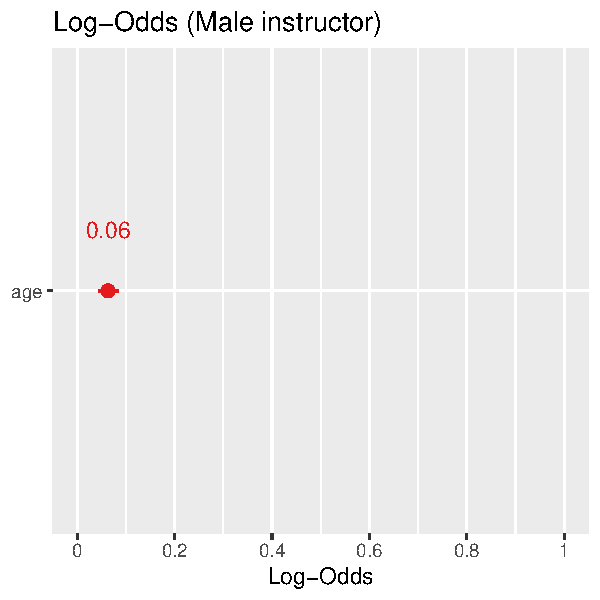
\includegraphics{index_files/figure-pdf/unnamed-chunk-15-1.pdf}

}

\caption{The log-odds of age for male instructors.}

\end{figure}%

Some of the interesting arguments that can be passed to the
\texttt{plot\_model} function are:

\begin{itemize}
\tightlist
\item
  \texttt{show.values\ =\ TRUE/FALSE}: Whether the log-odds/odds values
  should be displayed;
\item
  \texttt{show.p\ =\ TRUE/FALSE}: Adds asterisks that indicate the
  significance level of estimates to the value labels;
\item
  \texttt{transform}: A character vector naming the function that will
  be applied to the estimates. The default transformation uses
  \texttt{exp} to display the odds ratios, while
  \texttt{transform\ =\ NULL} displays the log-odds; and
\item
  \texttt{vline.color}: colour of the vertical ``zero effect'' line.
\end{itemize}

Further details on using \texttt{plot\_model} can be found
\href{https://strengejacke.wordpress.com/2017/10/23/one-function-to-rule-them-all-visualization-of-regression-models-in-rstats-w-sjplot/}{here}.

\begin{tcolorbox}[enhanced jigsaw, colframe=quarto-callout-warning-color-frame, toprule=.15mm, toptitle=1mm, opacitybacktitle=0.6, breakable, colback=white, opacityback=0, title={Task}, rightrule=.15mm, bottomrule=.15mm, coltitle=black, colbacktitle=quarto-callout-warning-color!10!white, leftrule=.75mm, left=2mm, arc=.35mm, bottomtitle=1mm, titlerule=0mm]

Produce a 95\% Wald confidence interval (i.e., based on asymptotic
normality) for the age coefficient by ``hand'', i.e.~using only the
coefficient's estimate and std. error. Then compare this result with the
confidence interval obtained in R.

Notice that the \texttt{tidy} function will compute a confidence
interval using the profile-likelihood by default. Thus, if you want the
results to be comparable, you will need to use the
\texttt{confint.default()} function.

I need a hint

Recall that a 95\% Wald CI for \(\beta\) can be computed as
\(\hat{\beta} \pm z_{1-\alpha/2} \times SE(\hat{\beta})\), where
\(SE(\cdot)\) denotes the standard error of the estimate and
\(z_{1-\alpha/2}\) the quantile of the Normal density.

See the solution

\begin{Shaded}
\begin{Highlighting}[]
\NormalTok{mod.coef.logodds }\OtherTok{\textless{}{-}}\NormalTok{ model }\SpecialCharTok{\%\textgreater{}\%} \FunctionTok{tidy}\NormalTok{() }\SpecialCharTok{\%\textgreater{}\%} \FunctionTok{filter}\NormalTok{(term}\SpecialCharTok{==}\StringTok{"age"}\NormalTok{)}

\CommentTok{\# Compute Wald 95\% CI by hand}
\NormalTok{mod.coef.logodds}\SpecialCharTok{$}\NormalTok{estimate }\SpecialCharTok{+}\NormalTok{ (}\FunctionTok{c}\NormalTok{(}\SpecialCharTok{{-}}\DecValTok{1}\NormalTok{,}\DecValTok{1}\NormalTok{)}\SpecialCharTok{*}
\FunctionTok{qnorm}\NormalTok{(}\FloatTok{0.975}\NormalTok{)) }\SpecialCharTok{*}\NormalTok{ mod.coef.logodds}\SpecialCharTok{$}\NormalTok{std.error }
\end{Highlighting}
\end{Shaded}

\begin{verbatim}
[1] 0.04221815 0.08371129
\end{verbatim}

\begin{Shaded}
\begin{Highlighting}[]
\CommentTok{\# Compare with Wald 95\% CI in R}
\FunctionTok{confint.default}\NormalTok{(model)[}\DecValTok{2}\NormalTok{,]}
\end{Highlighting}
\end{Shaded}

\begin{verbatim}
     2.5 %     97.5 % 
0.04221815 0.08371129 
\end{verbatim}

\end{tcolorbox}

\subsection{Odds}\label{odds}

Typically we would like to work on the \textbf{odds} scale as it is
easier to interpret. To obtain the odds we simply exponentiate the
log-odds, that is

\begin{align}
\frac{p}{1-p} &= \exp\left(\alpha + \beta \cdot \textrm{age} \right), \nonumber
\end{align}

When using the \texttt{tab\_model} function we simply set
\texttt{transform\ =\ "exp"}

\begin{Shaded}
\begin{Highlighting}[]
\NormalTok{model }\SpecialCharTok{\%\textgreater{}\%} \FunctionTok{tab\_model}\NormalTok{(}\AttributeTok{transform =} \StringTok{"exp"}\NormalTok{,}\AttributeTok{show.ci =} \ConstantTok{NULL}\NormalTok{)}
\end{Highlighting}
\end{Shaded}

\begin{longtable}[]{@{}ccc@{}}
\toprule\noalign{}
\endhead
\bottomrule\noalign{}
\endlastfoot
~ & \multicolumn{2}{c@{}}{%
gender} \\
Predictors & Odds Ratios & p \\
(Intercept) & 0.07 & \textbf{\textless0.001} \\
age & 1.06 & \textbf{\textless0.001} \\
Observations & \multicolumn{2}{l@{}}{%
463} \\
R\textsuperscript{2} Tjur & \multicolumn{2}{l@{}}{%
0.079} \\
\end{longtable}

Alternatively, for a \texttt{data.frame} output via the \texttt{tidy}
function we use:

\begin{Shaded}
\begin{Highlighting}[]
\NormalTok{model }\SpecialCharTok{\%\textgreater{}\%}\NormalTok{ broom}\SpecialCharTok{::}\FunctionTok{tidy}\NormalTok{(}\AttributeTok{exponentiate =}\NormalTok{ T)}
\end{Highlighting}
\end{Shaded}

\begin{verbatim}
# A tibble: 2 x 5
  term        estimate std.error statistic       p.value
  <chr>          <dbl>     <dbl>     <dbl>         <dbl>
1 (Intercept)   0.0673    0.512      -5.27 0.000000136  
2 age           1.06      0.0106      5.95 0.00000000271
\end{verbatim}

\begin{itemize}
\item
  On the odds scale, the value of the intercept (0.07) gives the odds of
  a teaching instructor being male given their \texttt{age\ =\ 0}, which
  is obviously not a viable age for a teaching instructor, and hence why
  this value is very close to zero.
\item
  For \texttt{age} we have an odds of 1.06, which indicates that for
  every 1 unit increase in age, the odds of the teaching instructor
  being male increase by a factor of 1.06 (equivalently to say that the
  odds of being a male are 6\% greater than a female for every unit
  increase in age).
\end{itemize}

For example, the odds of a teaching instructor who is 45 years old being
male is given by

\begin{align} \text{Odds}(\text{male|age=45}) &= \frac{p_{(\text{age=45})}}{1-p_{(\text{age=45})}} \\
&= \exp\left(\alpha + \beta \cdot \textrm{age = 45}\right) \\
&= \exp\left(-2.7 + 0.06 \cdot 45\right) = 1.15. \nonumber \end{align}

This can be interpreted as the chances of an instructor who is 45 being
male are 15\% greater than them being female (Note that
\(p_{(\text{age=45})}= \text{Prob}(\text{Male =1 | age =45})\)).

\textbf{Odds ratio}

How is the coefficient associated with age calculated? Let's look at the
\textbf{odds-ratio} obtained by comparing the odds of instructors aged
51 and 52 years old, that is, a one unit difference:

\begin{align}
\frac{\text{Odds}(\text{male|age=52})}{\text{Odds}(\text{male|age=51})} &= \left(\frac{\frac{p_{\text{age=52}}}{1 - p_{\text{age=52}}}}{\frac{p_{\text{age=51}}}{1 - p_{\text{age=51}}}}\right) \\
&= \frac{\exp\left(\alpha + \beta \cdot 52\right)}{\exp\left(\alpha + \beta \cdot 51\right)} = \exp\left(\beta \cdot (52 - 51)\right) \\
&= \exp\left(0.06\right) = 1.06. \nonumber
\end{align}

Which is exactly the estimate we get in
Table~\ref{tbl-summaries_Odds_conti} below.

Lastly, we can obtain a 95\% confidence interval for the odds by simply
exponentiating the lower and upper bounds of our log-odds interval:

\begin{Shaded}
\begin{Highlighting}[]
\NormalTok{model }\SpecialCharTok{\%\textgreater{}\%} \FunctionTok{tab\_model}\NormalTok{(}\AttributeTok{transform =} \StringTok{"exp"}\NormalTok{,}\AttributeTok{show.ci =} \FloatTok{0.95}\NormalTok{) }
\end{Highlighting}
\end{Shaded}

\begin{longtable}[]{@{}cccc@{}}

\caption{\label{tbl-summaries_Odds_conti}Logistic regression with a
continuous covariate odd-scale estimates}

\tabularnewline

\toprule\noalign{}
\endhead
\bottomrule\noalign{}
\endlastfoot
~ & \multicolumn{3}{c@{}}{%
gender} \\
Predictors & Odds Ratios & CI & p \\
(Intercept) & 0.07 & 0.02~--~0.18 & \textbf{\textless0.001} \\
age & 1.06 & 1.04~--~1.09 & \textbf{\textless0.001} \\
Observations & \multicolumn{3}{l@{}}{%
463} \\
R\textsuperscript{2} Tjur & \multicolumn{3}{l@{}}{%
0.079} \\

\end{longtable}

\begin{Shaded}
\begin{Highlighting}[]
\NormalTok{model }\SpecialCharTok{\%\textgreater{}\%}\NormalTok{ broom}\SpecialCharTok{::}\FunctionTok{tidy}\NormalTok{(}\AttributeTok{exponentiate =}\NormalTok{ T,}\AttributeTok{conf.int =}\NormalTok{ T) }
\end{Highlighting}
\end{Shaded}

\begin{longtable}[]{@{}
  >{\raggedright\arraybackslash}p{(\columnwidth - 12\tabcolsep) * \real{0.1765}}
  >{\raggedleft\arraybackslash}p{(\columnwidth - 12\tabcolsep) * \real{0.1324}}
  >{\raggedleft\arraybackslash}p{(\columnwidth - 12\tabcolsep) * \real{0.1471}}
  >{\raggedleft\arraybackslash}p{(\columnwidth - 12\tabcolsep) * \real{0.1471}}
  >{\raggedleft\arraybackslash}p{(\columnwidth - 12\tabcolsep) * \real{0.1176}}
  >{\raggedleft\arraybackslash}p{(\columnwidth - 12\tabcolsep) * \real{0.1324}}
  >{\raggedleft\arraybackslash}p{(\columnwidth - 12\tabcolsep) * \real{0.1471}}@{}}
\toprule\noalign{}
\begin{minipage}[b]{\linewidth}\raggedright
term
\end{minipage} & \begin{minipage}[b]{\linewidth}\raggedleft
estimate
\end{minipage} & \begin{minipage}[b]{\linewidth}\raggedleft
std.error
\end{minipage} & \begin{minipage}[b]{\linewidth}\raggedleft
statistic
\end{minipage} & \begin{minipage}[b]{\linewidth}\raggedleft
p.value
\end{minipage} & \begin{minipage}[b]{\linewidth}\raggedleft
conf.low
\end{minipage} & \begin{minipage}[b]{\linewidth}\raggedleft
conf.high
\end{minipage} \\
\midrule\noalign{}
\endhead
\bottomrule\noalign{}
\endlastfoot
(Intercept) & 0.07 & 0.51 & -5.27 & 0 & 0.02 & 0.18 \\
age & 1.06 & 0.01 & 5.95 & 0 & 1.04 & 1.09 \\
\end{longtable}

Hence the point estimate for the odds is 1.06, which has a corresponding
95\% confidence interval of (1.04, 1.09). This can be displayed
graphically using the \texttt{plot\_model} function from the
\texttt{sjPlot} package by simply passing our \texttt{model} as an
argument as well as removing \texttt{transform\ =\ NULL} (the default
transformation is exponential):

\begin{Shaded}
\begin{Highlighting}[]
\FunctionTok{plot\_model}\NormalTok{(model, }\AttributeTok{show.values =} \ConstantTok{TRUE}\NormalTok{,}
           \AttributeTok{title =} \StringTok{"Odds (Male instructor)"}\NormalTok{, }\AttributeTok{show.p =} \ConstantTok{FALSE}\NormalTok{, }\AttributeTok{axis.lim =} \FunctionTok{c}\NormalTok{(}\DecValTok{1}\NormalTok{, }\FloatTok{1.5}\NormalTok{))}
\end{Highlighting}
\end{Shaded}

\begin{figure}[H]

{\centering 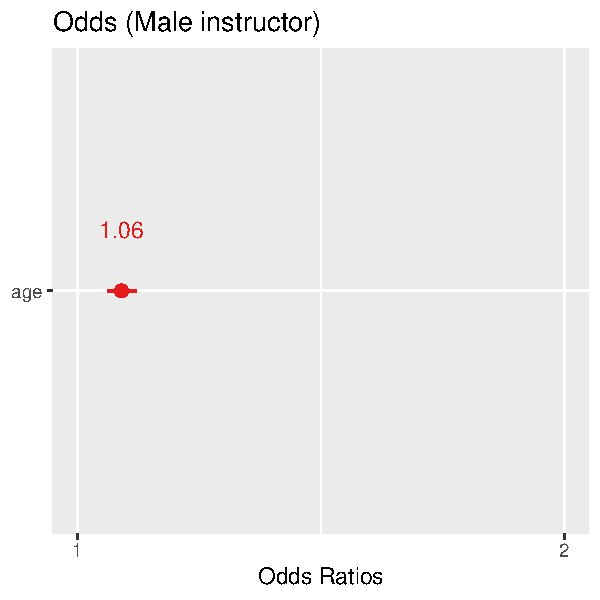
\includegraphics{index_files/figure-pdf/unnamed-chunk-22-1.pdf}

}

\caption{The odds of age for male instructors.}

\end{figure}%

\textbf{Note}: \texttt{axis.lim} is used to zoom in on the 95\%
confidence interval.

\subsection{Probabilities}\label{probabilities}

Since we have used the logit link function to link the linear predictor
\(\alpha + \beta \cdot \textrm{age}\) to the probabilities of being a
male, we can then obtain back the probability
\(p = \textrm{Prob}(\textrm{Male})\) by using the inverse-logit
transformation:

\begin{align}
p &= \frac{\exp\left(\alpha + \beta \cdot \textrm{age} \right)}{1 + \exp\left(\alpha + \beta \cdot \textrm{age} \right)} . \nonumber
\end{align}

For example, the probability of a teaching instructor who is 52 years
old being male is

\begin{align}
p &= \frac{\exp\left(\alpha + \beta \cdot \textrm{age} \right)}{1 + \exp\left(\alpha + \beta \cdot \textrm{age} \right)}
=\frac{\exp\left(-2.7 + 0.06\cdot 52 \right)}{1 + \exp\left(-2.7 + 0.06\cdot 52 \right)} 
= 0.64, \nonumber
\end{align}

which can be computed in R using the inverse logit \texttt{plogis()}
function from the \texttt{stats} library:

\begin{Shaded}
\begin{Highlighting}[]
\FunctionTok{plogis}\NormalTok{(model}\SpecialCharTok{$}\NormalTok{coefficients[}\DecValTok{1}\NormalTok{] }
              \SpecialCharTok{+}\NormalTok{ model}\SpecialCharTok{$}\NormalTok{coefficients[}\DecValTok{2}\NormalTok{] }\SpecialCharTok{*}  \DecValTok{52}\NormalTok{)}
\end{Highlighting}
\end{Shaded}

\begin{verbatim}
(Intercept) 
  0.6401971 
\end{verbatim}

Finally, we can plot the probability of being male using \texttt{sjPlot}
by specifying the following:

\begin{enumerate}
\def\labelenumi{\arabic{enumi}.}
\item
  The model we have fitted
\item
  \texttt{type\ =\ "pred"} to plot predicted values (marginal effects)
  for specific model terms.
\item
  The model terms of interest. Here, you can also plot the marginal
  effects at specific values ,e.g.~selecting \texttt{age{[}30:60{]}}
  will plot the predictions based on age-values from 30 to 60, while
  \texttt{age{[}all{]}} will plot the predictions across all of the
  range of our independent variable (You can also provide a custom grid
  to evaluate you predictions, we will this cover next week).
\end{enumerate}

\begin{Shaded}
\begin{Highlighting}[]
\FunctionTok{plot\_model}\NormalTok{(model, }
           \AttributeTok{type =} \StringTok{"pred"}\NormalTok{, }
           \AttributeTok{title =} \StringTok{""}\NormalTok{, }
           \AttributeTok{terms=}\StringTok{"age [all]"}\NormalTok{, }
           \AttributeTok{axis.title =} \FunctionTok{c}\NormalTok{(}\StringTok{"Age"}\NormalTok{, }\StringTok{"Prob. of instructor being male"}\NormalTok{))}
\end{Highlighting}
\end{Shaded}

\begin{figure}[H]

{\centering 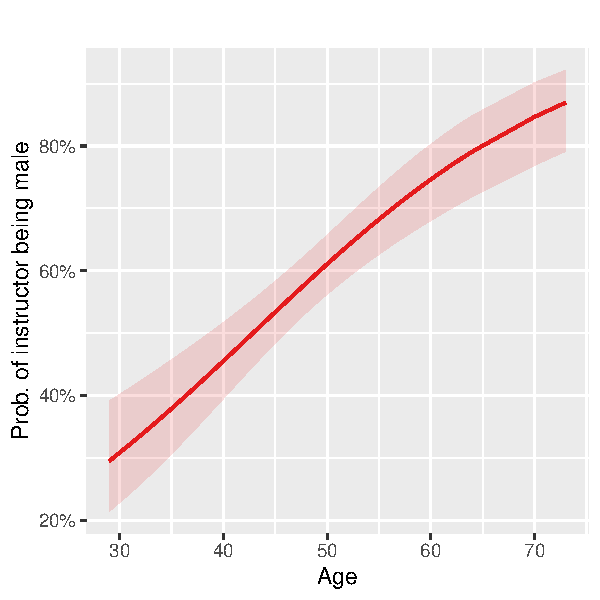
\includegraphics{index_files/figure-pdf/unnamed-chunk-24-1.pdf}

}

\caption{Probability of teaching instructor being male by age.}

\end{figure}%

Table~\ref{tbl-odds_probs} summarises the relationship between between
Odds and Probabilities:

\begin{longtable}[]{@{}
  >{\raggedright\arraybackslash}p{(\columnwidth - 2\tabcolsep) * \real{0.2083}}
  >{\raggedright\arraybackslash}p{(\columnwidth - 2\tabcolsep) * \real{0.7917}}@{}}
\caption{Relationship between Odds and
Probabilities}\label{tbl-odds_probs}\tabularnewline
\toprule\noalign{}
\begin{minipage}[b]{\linewidth}\raggedright
Scale
\end{minipage} & \begin{minipage}[b]{\linewidth}\raggedright
Equivalence
\end{minipage} \\
\midrule\noalign{}
\endfirsthead
\toprule\noalign{}
\begin{minipage}[b]{\linewidth}\raggedright
Scale
\end{minipage} & \begin{minipage}[b]{\linewidth}\raggedright
Equivalence
\end{minipage} \\
\midrule\noalign{}
\endhead
\bottomrule\noalign{}
\endlastfoot
Odds &
\(                                                                                                                                                                                                                                                                                                                                                                                                                                                                   
                                                                                                                                                                                                                                                                                                                           Odds = \mathrm{exp}(log Odds) = \dfrac{P(event)}{1-P(event)}                                                                                              
                                                                                                                                                                                                                                                                                                                           \) \\
Probability &
\(                                                                                                                                                                                                                                                                                                                                                                                                                                                                   
                                                                                                                                                                                                                                                                                                                           P(event) =\dfrac{\mathrm{exp}(logOdds)}{1+\mathrm{exp}(logOdds)}  = \dfrac{Odds}{1+Odds}                                                                  
                                                                                                                                                                                                                                                                                                                           \) \\
\end{longtable}

\section{Model evaluation}\label{model-evaluation}

\subsection{Diagnostic plots}\label{diagnostic-plots}

As usual, now that we have fitted the model we need to assess how well
the model fits the data and check whether our assumptions are met. Our
assumptions can be checked as usual by using the \texttt{plot()}
function in base R. However, we can visualize this with a much nicer and
appropiate layout using the \texttt{check\_model()} function within the
\texttt{performance} library.

\begin{Shaded}
\begin{Highlighting}[]
\FunctionTok{library}\NormalTok{(performance)}
\FunctionTok{check\_model}\NormalTok{(model, }\AttributeTok{check =} \FunctionTok{c}\NormalTok{(}\StringTok{"pp\_check"}\NormalTok{,}\StringTok{"binned\_residuals"}\NormalTok{,}\StringTok{"outliers"}\NormalTok{,}\StringTok{"qq"}\NormalTok{))}
\end{Highlighting}
\end{Shaded}

\begin{figure}[H]

{\centering 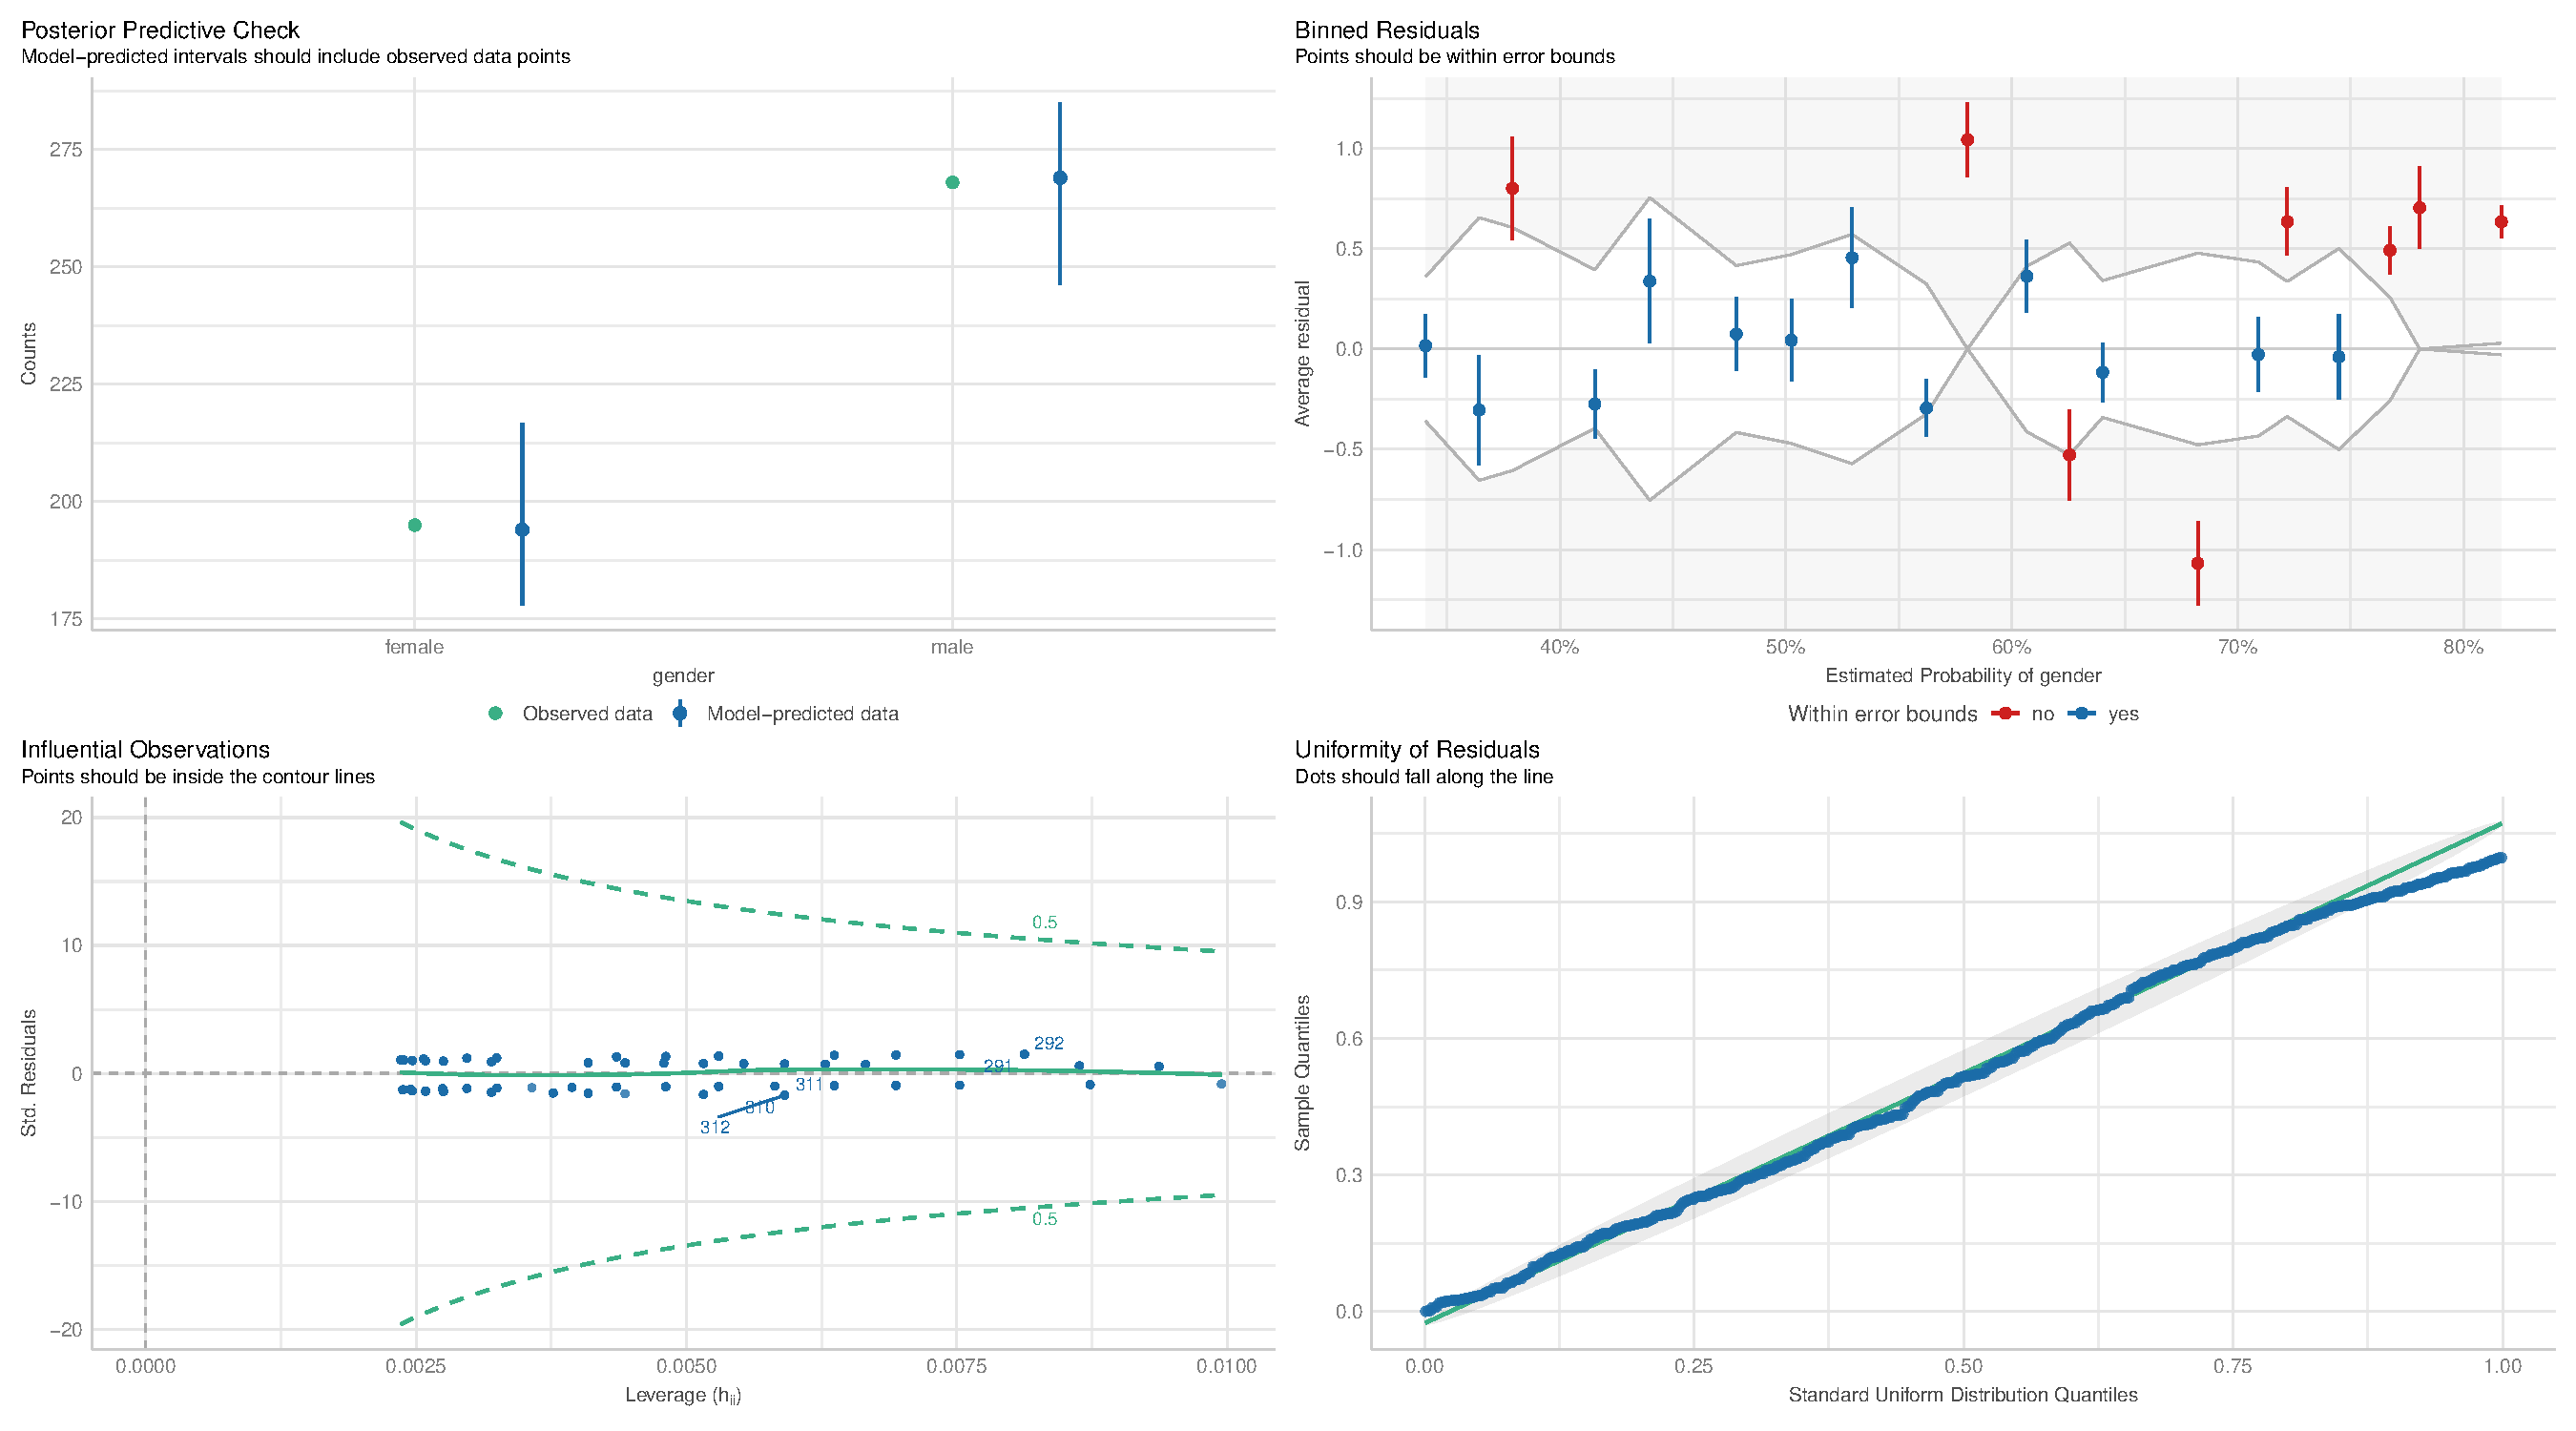
\includegraphics{index_files/figure-pdf/unnamed-chunk-25-1.pdf}

}

\caption{GLM diagnostics for the gender of teaching instructors}

\end{figure}%

\begin{tcolorbox}[enhanced jigsaw, colframe=quarto-callout-caution-color-frame, toprule=.15mm, toptitle=1mm, opacitybacktitle=0.6, breakable, colback=white, opacityback=0, title=\textcolor{quarto-callout-caution-color}{\faFire}\hspace{0.5em}{Caution}, rightrule=.15mm, bottomrule=.15mm, coltitle=black, colbacktitle=quarto-callout-caution-color!10!white, leftrule=.75mm, left=2mm, arc=.35mm, bottomtitle=1mm, titlerule=0mm]

Be aware that the \texttt{performance} library has quite a few
dependencies so check whether any package needs to be updated when you
install the package for the first time.

\end{tcolorbox}

The output shows us 4 different diagnostic plots. These are:

\begin{enumerate}
\def\labelenumi{\arabic{enumi}.}
\item
  \textbf{Posterior predictive check} (Top-left): Compares the observed
  data (in this case the number of females and males) against the
  predicted number of males and females using simulated data. We can
  look for systematic discrepancies between real and simulated data to
  assess the goodness of fit (see. (Gabry et al. 2019) and
  \texttt{check\_predictions()} for further details)
\item
  \textbf{Binned residuals} (Top-right): Bin the observations based on
  their fitted values, and average the residual value in each bin. The
  plots shows the average residual values versus the average fitted
  value for each bin'' (Gelman and Hill 2006). If the model were true,
  one would expect about 95\% of the residuals to fall inside the error
  bounds (see \texttt{?binned\_residuals} for more details.)
\item
  \textbf{Influential observations} (Bottom-left): This plot is used to
  identify influential observations. If any points in this plot fall
  outside of Cook's distance (the dashed lines) then it is considered an
  influential observation. See \texttt{check\_outliers()} for further
  details.
\item
  \textbf{Uniformity of residuals} (Bottom-right): Since our response is
  not normally distributed, residuals are not expected to be normally
  distributed either. Thus, we can use QQ plots to check the uniformity
  of residuals, i.e.~the extent to which the observed values deviate
  from the model expectations using simulated residuals instead of the
  usual Pearson residuals
\end{enumerate}

\subsection{Predictive performance
metrics}\label{predictive-performance-metrics}

Since our outcome of interest is a binary categorical variable, we can
compute the predicted classes and evaluate how accurate our predictions
are by comparing them against the observed values. To do so, we can add
the predicted (fitted) values to our data with \texttt{broom::augment()}
and classify them based on a decision threshold.

\begin{tcolorbox}[enhanced jigsaw, colframe=quarto-callout-note-color-frame, toprule=.15mm, toptitle=1mm, opacitybacktitle=0.6, breakable, colback=white, opacityback=0, title=\textcolor{quarto-callout-note-color}{\faInfo}\hspace{0.5em}{Note}, rightrule=.15mm, bottomrule=.15mm, coltitle=black, colbacktitle=quarto-callout-note-color!10!white, leftrule=.75mm, left=2mm, arc=.35mm, bottomtitle=1mm, titlerule=0mm]

Note that we can append either the logit-scaled fitted values (by
setting \texttt{type.predict\ =\ c("link")} or the predicted
probabilities (\texttt{type.predict\ =\ c("response")}).

\end{tcolorbox}

In the case of logistic regression, you typically classify these
probabilities into discrete classes based on a cutoff (commonly 0.5 for
binary classification). Here is an example where predicted probabilities
outcomes of \(\hat{p} > 0.5\) are classified as \texttt{male} and as
\texttt{female} if \(\hat{p} \leq 0.5\) .

\begin{Shaded}
\begin{Highlighting}[]
\NormalTok{pred\_results }\OtherTok{=}\NormalTok{ model }\SpecialCharTok{\%\textgreater{}\%} 
\NormalTok{  broom}\SpecialCharTok{::}\FunctionTok{augment}\NormalTok{(}\AttributeTok{type.predict =} \FunctionTok{c}\NormalTok{(}\StringTok{"response"}\NormalTok{)) }\SpecialCharTok{\%\textgreater{}\%}
  \FunctionTok{mutate}\NormalTok{(}\AttributeTok{predicted\_class =} 
           \FunctionTok{factor}\NormalTok{(}\FunctionTok{ifelse}\NormalTok{(.fitted }\SpecialCharTok{\textgreater{}} \FloatTok{0.5}\NormalTok{, }\StringTok{"male"}\NormalTok{, }\StringTok{"female"}\NormalTok{)))}
\end{Highlighting}
\end{Shaded}

\begin{longtable}[]{@{}
  >{\raggedright\arraybackslash}p{(\columnwidth - 16\tabcolsep) * \real{0.0795}}
  >{\raggedleft\arraybackslash}p{(\columnwidth - 16\tabcolsep) * \real{0.0455}}
  >{\raggedleft\arraybackslash}p{(\columnwidth - 16\tabcolsep) * \real{0.1136}}
  >{\raggedleft\arraybackslash}p{(\columnwidth - 16\tabcolsep) * \real{0.1250}}
  >{\raggedleft\arraybackslash}p{(\columnwidth - 16\tabcolsep) * \real{0.1136}}
  >{\raggedleft\arraybackslash}p{(\columnwidth - 16\tabcolsep) * \real{0.1023}}
  >{\raggedleft\arraybackslash}p{(\columnwidth - 16\tabcolsep) * \real{0.1136}}
  >{\raggedleft\arraybackslash}p{(\columnwidth - 16\tabcolsep) * \real{0.1250}}
  >{\raggedright\arraybackslash}p{(\columnwidth - 16\tabcolsep) * \real{0.1818}}@{}}
\toprule\noalign{}
\begin{minipage}[b]{\linewidth}\raggedright
gender
\end{minipage} & \begin{minipage}[b]{\linewidth}\raggedleft
age
\end{minipage} & \begin{minipage}[b]{\linewidth}\raggedleft
.fitted
\end{minipage} & \begin{minipage}[b]{\linewidth}\raggedleft
.resid
\end{minipage} & \begin{minipage}[b]{\linewidth}\raggedleft
.hat
\end{minipage} & \begin{minipage}[b]{\linewidth}\raggedleft
.sigma
\end{minipage} & \begin{minipage}[b]{\linewidth}\raggedleft
.cooksd
\end{minipage} & \begin{minipage}[b]{\linewidth}\raggedleft
.std.resid
\end{minipage} & \begin{minipage}[b]{\linewidth}\raggedright
predicted\_class
\end{minipage} \\
\midrule\noalign{}
\endhead
\bottomrule\noalign{}
\endlastfoot
female & 36 & 0.3938360 & -1.0006045 & 0.0058192 & 1.132909 & 0.0019126
& -1.003529 & female \\
female & 36 & 0.3938360 & -1.0006045 & 0.0058192 & 1.132909 & 0.0019126
& -1.003529 & female \\
female & 36 & 0.3938360 & -1.0006045 & 0.0058192 & 1.132909 & 0.0019126
& -1.003529 & female \\
female & 36 & 0.3938360 & -1.0006045 & 0.0058192 & 1.132909 & 0.0019126
& -1.003529 & female \\
male & 59 & 0.7343825 & 0.7857803 & 0.0047899 & 1.133280 & 0.0008746 &
0.787669 & male \\
\end{longtable}

We can use these predicted classes to compute different predictive
performance/evaluation metrics. To do so we can compute a confusion
matrix according to the true and predicted classes:

\begin{center}
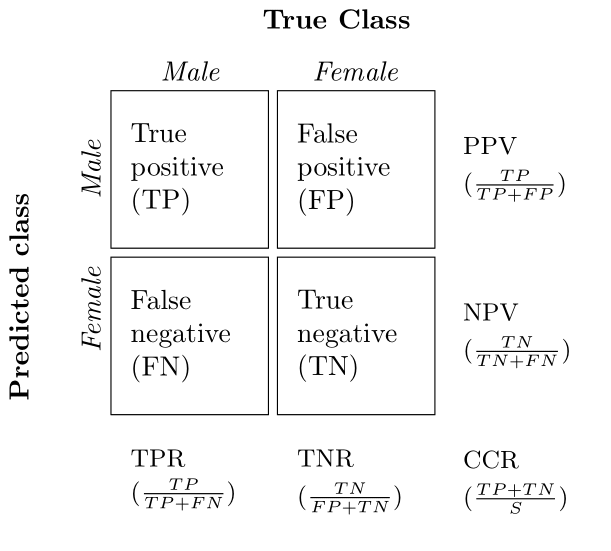
\includegraphics[width=4.79167in,height=\textheight]{tikz__pictures-1.png}
\end{center}

The table can be interpreted as follows:

\begin{itemize}
\item
  The \emph{correct classification rate} (CCR) or \emph{accuracy}
  describes the overall proportion of teaching instructors (males or
  females) that were classified correctly among all the \(S = 463\)
  individuals.
\item
  The \emph{true positive rate} (TPR) or \emph{sensitivity} (a.k.a.
  recall), denotes the proportion of actual male instructors that are
  correctly classified as males by the model.
\item
  The \emph{true negative rate} (TNR) or \emph{specificity}, denotes the
  proportion of actual females that have been classified correctly as
  females by the model. \textbf{Note}: the \emph{false positive rate}
  (FPR) computed as (1- \emph{specificity}) is another popular metric
  that measures the proportion of actual negatives that are incorrectly
  predicted as positive.
\item
  The model's \emph{precision} or \emph{positive predictive value} (PPV)
  represents the proportion of predicted male instructors that were
  actually male, i.e.~how many of the predicted positive cases were
  \textbf{actually positive}.
\item
  The model's \emph{negative predictive value} (NPV) represents the
  proportion of predicted female instructors that were actually females,
  i.e.~how many of the predicted negative cases were \textbf{actually
  negative}.
\end{itemize}

To compute the confusion matrix we can use the \texttt{conf\_mat()}
function from the \texttt{yardstick} package and use as input the data
frame with the predicted and observed classes as follows:

\begin{Shaded}
\begin{Highlighting}[]
\FunctionTok{library}\NormalTok{(yardstick)}
\FunctionTok{conf\_mat}\NormalTok{(pred\_results,}\AttributeTok{truth =}\NormalTok{ gender,}\AttributeTok{estimate =}\NormalTok{ predicted\_class)}
\end{Highlighting}
\end{Shaded}

\begin{verbatim}
          Truth
Prediction female male
    female     76   60
    male      119  208
\end{verbatim}

Rather than computing these predictive performance metrics by hand, we
can take advantage of the \texttt{metric\_set()} function from the
\texttt{yardstick} library to combine multiple metric functions together
into a new function that calculates all of them at once. Then we just
simply need to supply the same arguments we used for computing the
confusion matrix.

\begin{Shaded}
\begin{Highlighting}[]
\CommentTok{\# Step (1) create a set with classification metrics we want to compute}
\NormalTok{eval\_metric }\OtherTok{\textless{}{-}} \FunctionTok{metric\_set}\NormalTok{(accuracy,sensitivity,specificity,ppv,npv)}
\CommentTok{\# Step (2) call out the metric set and input the data containing the observed and predicted classes}
\FunctionTok{eval\_metric}\NormalTok{(pred\_results,}
            \AttributeTok{truth =}\NormalTok{ gender,}
            \AttributeTok{estimate =}\NormalTok{ predicted\_class,  }
            \AttributeTok{event\_level =} \StringTok{"second"}\NormalTok{) }
\end{Highlighting}
\end{Shaded}

\begin{longtable}[]{@{}llr@{}}
\toprule\noalign{}
.metric & .estimator & .estimate \\
\midrule\noalign{}
\endhead
\bottomrule\noalign{}
\endlastfoot
accuracy & binary & 0.61 \\
sensitivity & binary & 0.39 \\
specificity & binary & 0.78 \\
ppv & binary & 0.56 \\
npv & binary & 0.64 \\
\end{longtable}

\begin{tcolorbox}[enhanced jigsaw, colframe=quarto-callout-important-color-frame, toprule=.15mm, toptitle=1mm, opacitybacktitle=0.6, breakable, colback=white, opacityback=0, title=\textcolor{quarto-callout-important-color}{\faExclamation}\hspace{0.5em}{Important}, rightrule=.15mm, bottomrule=.15mm, coltitle=black, colbacktitle=quarto-callout-important-color!10!white, leftrule=.75mm, left=2mm, arc=.35mm, bottomtitle=1mm, titlerule=0mm]

Notice that we passed on the argument \texttt{event\_level\ =\ "second"}
since the default behavior of the \texttt{eval\_metric()} function
created via \texttt{metric\_set()} is to consider the first class of the
variable \texttt{gender}as the event. If you recall, \texttt{female}
appears as first due alphabetical order, and hence is treated as our
reference category in our model and thus we are modelling the event
\(\mathbb{Pr}(male)\)

\begin{Shaded}
\begin{Highlighting}[]
\FunctionTok{levels}\NormalTok{(pred\_results}\SpecialCharTok{$}\NormalTok{gender)}
\end{Highlighting}
\end{Shaded}

\begin{verbatim}
[1] "female" "male"  
\end{verbatim}

However since \texttt{female} appear first, we need to tell our function
that we are interested in the second class of the variables
\texttt{gender} , i.e.~\texttt{male}, as the event and not the other way
around.

\end{tcolorbox}

We can see that our model is not doing a great job in predicting the
outcome (accuracy of \(\approx\) 60\%).This is due to a particularly
poor performance in terms of \emph{specificity}, i.e.~roughly only 40\%
of truly male instructors are correctly classified as such by our mode.
Despite this, our model is not doing a terrible job in terms of
\emph{sensitivity} since almost 80\% of the females are actually being
predicted as such.

Note that the threshold of 0.5 is common but may not always be optimal.
You can adjust it based on your specific application and the desired
balance between sensitivity and specificity (we will see an example of
such in the next task).

\begin{tcolorbox}[enhanced jigsaw, colframe=quarto-callout-note-color-frame, toprule=.15mm, toptitle=1mm, opacitybacktitle=0.6, breakable, colback=white, opacityback=0, title=\textcolor{quarto-callout-note-color}{\faInfo}\hspace{0.5em}{Note}, rightrule=.15mm, bottomrule=.15mm, coltitle=black, colbacktitle=quarto-callout-note-color!10!white, leftrule=.75mm, left=2mm, arc=.35mm, bottomtitle=1mm, titlerule=0mm]

For this course we have been using only our data to assess the
predicative performance of our models. In reality, if we were to
properly assess the classification performance of our models, we should
look at out-of-sample prediction by first splitting the data into a
training and a test set, then fitting the model to the training data and
finally predicting the class of the each observation in the test data
that has been held back. Otherwise we run the risk of overstating the
classification accuracy of the model.

\end{tcolorbox}

\subsection{ROC Curve}\label{roc-curve}

Another way to assess how good the model is at separating the 2 classes
of the outcome is through the Receiver Operating Characteristic (ROC)
curve. The ROC curve is a graphical representation used to evaluate the
performance of a binary classification model. It shows the trade-off
between the true positive rate (sensitivity) and the false positive rate
(1 - specificity) at various threshold settings.

The threshold determines the cutoff probability for classifying a sample
as positive or negative (male or female in our case).

\begin{itemize}
\item
  At a cutoff \(=0\) , all the observations will be classified as
  positive (i.e.~all the instructors are going to be classified as males
  since we are modelling the event \(P(male)\)).
\item
  At a cutoff \(=1\) , all the observations will be classified as
  negative (i.e.~all the instructors are going to be classified as
  females corresponding to \(1 - P(male)\)).
\end{itemize}

As the threshold moves between 0 and 1, the ROC curve traces out points
that show the model's performance for various balances between TPR and
FPR.

We can combine the \texttt{roc\_curve()} function from the
\texttt{yardstick} library and \texttt{autoplot()} function from
\texttt{ggplot} to calculate and visualize the ROC curve. We just need
to supply the true classes and the predicted \textbf{probabilities} (NOT
the predicted \textbf{classes}!).

\begin{Shaded}
\begin{Highlighting}[]
\FunctionTok{roc\_curve}\NormalTok{(pred\_results,}
          \AttributeTok{truth =}\NormalTok{ gender,}
\NormalTok{          .fitted,}
          \AttributeTok{event\_level =} \StringTok{"second"}\NormalTok{) }\SpecialCharTok{\%\textgreater{}\%}
  \FunctionTok{autoplot}\NormalTok{()}
\end{Highlighting}
\end{Shaded}

\begin{figure}[H]

{\centering 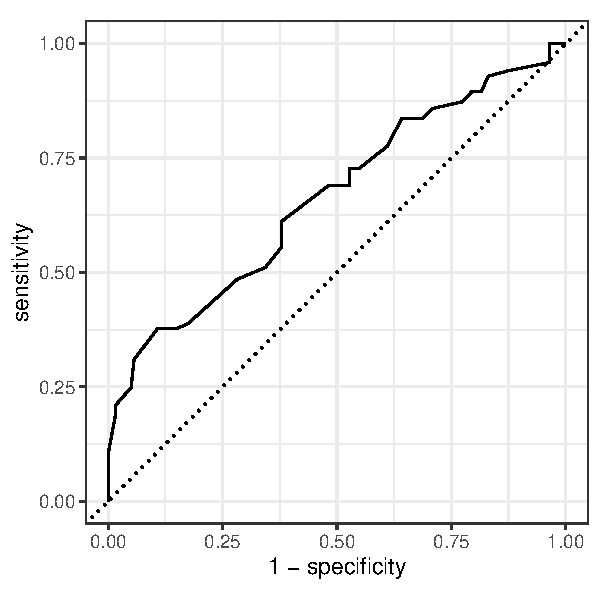
\includegraphics{index_files/figure-pdf/unnamed-chunk-35-1.pdf}

}

\caption{ROC curve for GLM fitted to the evaluation scores data set.}

\end{figure}%

\begin{tcolorbox}[enhanced jigsaw, colframe=quarto-callout-important-color-frame, toprule=.15mm, toptitle=1mm, opacitybacktitle=0.6, breakable, colback=white, opacityback=0, title=\textcolor{quarto-callout-important-color}{\faExclamation}\hspace{0.5em}{Important}, rightrule=.15mm, bottomrule=.15mm, coltitle=black, colbacktitle=quarto-callout-important-color!10!white, leftrule=.75mm, left=2mm, arc=.35mm, bottomtitle=1mm, titlerule=0mm]

Similarly to the the evaluation metric function we had before, we set
\texttt{event\_level\ =\ "second"} since the default behavior of the
\texttt{roc\_auc()} function is also to consider the first class of the
variable \texttt{gender}as the event. Thus, we need to tell the
\texttt{roc\_auc()} that we are interested in the \texttt{male} level as
our event, which is the second class of the variable \texttt{gender}.

\end{tcolorbox}

The closer the ROC curve is to the top-left corner, the better the model
is at distinguishing between the positive and negative classes. This
means high true positive rates (sensitivity) and low false positive
rates. The closer the curve is to the diagonal line (i.e.~when TPR =
FPR) then the performance is no better than random guessing. We can see
here that our model is doing a little bit better than just random
guessing.

We can also calculate the area under the ROC curve (AUC) as a single
value to summarize the model's performance:

\begin{Shaded}
\begin{Highlighting}[]
\NormalTok{yardstick}\SpecialCharTok{::}\FunctionTok{roc\_auc}\NormalTok{(pred\_results,}
        \AttributeTok{truth =}\NormalTok{ gender,}
\NormalTok{        .fitted,}
        \AttributeTok{event\_level =} \StringTok{"second"}\NormalTok{)}
\end{Highlighting}
\end{Shaded}

\begin{longtable}[]{@{}llr@{}}
\toprule\noalign{}
.metric & .estimator & .estimate \\
\midrule\noalign{}
\endhead
\bottomrule\noalign{}
\endlastfoot
roc\_auc & binary & 0.66 \\
\end{longtable}

The AUC ranges from 0 to 1:

\begin{itemize}
\item
  \textbf{AUC = 1}: Perfect classifier.
\item
  \textbf{AUC = 0.5}: No better than random guessing.
\item
  \textbf{AUC} \(\leq\) \textbf{0.5}: Worse than random guessing,
  meaning the model is consistently misclassifying.
\end{itemize}

Again, the AUC of 0.66 indicates a moderate-poor fit to the data (mainly
due to miss-classifications of male instructors as we saw previously).

\begin{tcolorbox}[enhanced jigsaw, colframe=quarto-callout-warning-color-frame, toprule=.15mm, toptitle=1mm, opacitybacktitle=0.6, breakable, colback=white, opacityback=0, title={Task}, rightrule=.15mm, bottomrule=.15mm, coltitle=black, colbacktitle=quarto-callout-warning-color!10!white, leftrule=.75mm, left=2mm, arc=.35mm, bottomtitle=1mm, titlerule=0mm]

The \textbf{Youden} index (\emph{Youden's J statistics}) is a summary
metric that helps to identify the optimal threshold that maximizes both
sensitivity (true positive rate) and specificity (true negative rate)
simultaneously. It is computed as follows:

\[ J = \mathrm{sensitivity} + \mathrm{specificity} -1 \]

Compute the Youden index and find the optimal threshold that maximizes
both sensitivity and specificity in the logistic regression model fitted
to the evaluation scores data set.

Take hint

You can use the \texttt{roc\_curve()} function to compute the
sensitivity and specificity values at different thresholds. Then use
these values to compute Youden's index and find the threshold value
associated with the maximum value of Youden's index.

Click here to see the solution

\begin{Shaded}
\begin{Highlighting}[]
\FunctionTok{roc\_curve}\NormalTok{(pred\_results,}
          \AttributeTok{truth =}\NormalTok{ gender,}
\NormalTok{          .fitted,}
          \AttributeTok{event\_level =} \StringTok{"second"}\NormalTok{) }\SpecialCharTok{\%\textgreater{}\%} 
  \FunctionTok{mutate}\NormalTok{(}\AttributeTok{youden\_j =}\NormalTok{ sensitivity }\SpecialCharTok{+}\NormalTok{ specificity }\SpecialCharTok{{-}} \DecValTok{1}\NormalTok{) }\SpecialCharTok{\%\textgreater{}\%} 
  \FunctionTok{filter}\NormalTok{(youden\_j }\SpecialCharTok{==} \FunctionTok{max}\NormalTok{(youden\_j)) }\SpecialCharTok{\%\textgreater{}\%} 
  \FunctionTok{select}\NormalTok{(.threshold)}
\end{Highlighting}
\end{Shaded}

\begin{verbatim}
# A tibble: 1 x 1
  .threshold
       <dbl>
1      0.709
\end{verbatim}

\end{tcolorbox}

\section{Logistic regression with one categorical explanatory
variable}\label{logistic-regression-with-one-categorical-explanatory-variable}

Instead of having a numerical explanatory variable such as \texttt{age},
let's now use the binary categorical variable \texttt{ethnicity} as our
explanatory variable.

\begin{Shaded}
\begin{Highlighting}[]
\NormalTok{evals.ethnic }\OtherTok{\textless{}{-}}\NormalTok{ evals }\SpecialCharTok{\%\textgreater{}\%}
                  \FunctionTok{select}\NormalTok{(gender, ethnicity)}
\end{Highlighting}
\end{Shaded}

\begin{longtable}[]{@{}ll@{}}
\toprule\noalign{}
gender & ethnicity \\
\midrule\noalign{}
\endhead
\bottomrule\noalign{}
\endlastfoot
female & minority \\
female & minority \\
female & minority \\
female & minority \\
male & not minority \\
\end{longtable}

Now, let's look at a barplot of the proportion of males and females by
\texttt{ethnicity} to get an initial impression of the data.

\begin{tcolorbox}[enhanced jigsaw, colframe=quarto-callout-tip-color-frame, toprule=.15mm, toptitle=1mm, opacitybacktitle=0.6, breakable, colback=white, opacityback=0, title=\textcolor{quarto-callout-tip-color}{\faLightbulb}\hspace{0.5em}{Tip}, rightrule=.15mm, bottomrule=.15mm, coltitle=black, colbacktitle=quarto-callout-tip-color!10!white, leftrule=.75mm, left=2mm, arc=.35mm, bottomtitle=1mm, titlerule=0mm]

We can also use the \texttt{tabyl} function from the \texttt{janitor}
package to display percentage data in an organized way. See
\texttt{?tabyl} for more details.

\begin{Shaded}
\begin{Highlighting}[]
\FunctionTok{library}\NormalTok{(janitor)}
\NormalTok{evals.ethnic }\SpecialCharTok{\%\textgreater{}\%}
  \FunctionTok{tabyl}\NormalTok{(ethnicity, gender) }\SpecialCharTok{\%\textgreater{}\%}
  \FunctionTok{adorn\_percentages}\NormalTok{() }\SpecialCharTok{\%\textgreater{}\%}
  \FunctionTok{adorn\_pct\_formatting}\NormalTok{() }\SpecialCharTok{\%\textgreater{}\%}
  \FunctionTok{adorn\_ns}\NormalTok{() }\CommentTok{\# To show original counts}
\end{Highlighting}
\end{Shaded}

\begin{verbatim}
    ethnicity      female        male
     minority 56.2%  (36) 43.8%  (28)
 not minority 39.8% (159) 60.2                                        (240)
\end{verbatim}

\end{tcolorbox}

\section{R plot}

\begin{figure}[H]

{\centering 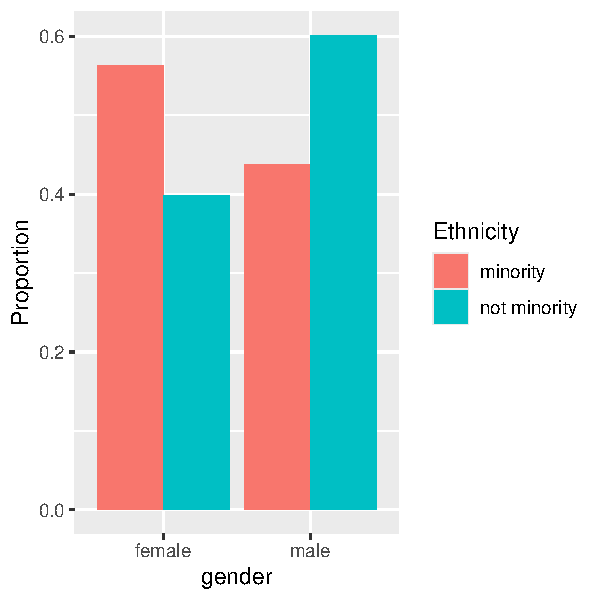
\includegraphics{index_files/figure-pdf/unnamed-chunk-42-1.pdf}

}

\caption{Barplot of teaching instructors' gender by ethnicity.}

\end{figure}%

\section{R Code}

\begin{Shaded}
\begin{Highlighting}[]
\FunctionTok{ggplot}\NormalTok{(evals.ethnic, }\FunctionTok{aes}\NormalTok{(}\AttributeTok{x =}\NormalTok{ gender, }\AttributeTok{group =}\NormalTok{ ethnicity)) }\SpecialCharTok{+}
    \FunctionTok{geom\_bar}\NormalTok{(}\FunctionTok{aes}\NormalTok{(}\AttributeTok{y =} \FunctionTok{after\_stat}\NormalTok{(prop), }\AttributeTok{fill =}\NormalTok{ ethnicity), }
             \AttributeTok{stat =} \StringTok{"count"}\NormalTok{, }\AttributeTok{position =} \StringTok{"dodge"}\NormalTok{) }\SpecialCharTok{+}
    \FunctionTok{labs}\NormalTok{(}\AttributeTok{y =} \StringTok{"Proportion"}\NormalTok{, }\AttributeTok{fill =} \StringTok{"Ethnicity"}\NormalTok{)}
\end{Highlighting}
\end{Shaded}

We can see that a larger proportion of instructors in the
\texttt{minority} ethnic group are female (56.3\% vs 43.8\%), while the
\texttt{not\ minority} ethnic group is comprised of more male
instructors (60.2\% vs 39.8\%). Now we shall fit a logistic regression
model to determine whether the gender of a teaching instructor can be
predicted from their ethnicity.

\subsection{Log-odds}\label{log-odds-1}

The logistic regression model is given by:

\begin{align}
y_i &\sim \mathrm{Bernoulli}(p_i)\\
\mathrm{logit}(p_i) &= \alpha +  \beta_{\text{ethnicity}}  \times \mathbb{I}_{\text{ethnicity}}(\mathrm{not~  minority}).
\end{align}

Which can be fitted in R as follows:

\begin{Shaded}
\begin{Highlighting}[]
\NormalTok{model.ethnic }\OtherTok{\textless{}{-}} \FunctionTok{glm}\NormalTok{(gender }\SpecialCharTok{\textasciitilde{}}\NormalTok{ ethnicity,}
                    \AttributeTok{data =}\NormalTok{ evals.ethnic,}
                    \AttributeTok{family =}\NormalTok{ binomial) }
\end{Highlighting}
\end{Shaded}

Here, \(y_i\) denotes the \(i\)th instructor's gender, again, the
baseline category for our binary response is \texttt{female}. Thus,
\(p_i = \mathrm{Prob}(\mathrm{Male})\) is linked to the linear predictor
through the logit link function. This means that estimates we get from
fitting the logistic regression model are for a change on the
\textbf{log-odds} scale for \texttt{males}
(\(p_i = \textrm{Prob}(\textrm{Males})\)) in comparison to the response
baseline \texttt{females}.

Also, the baseline category for our explanatory variable is
\texttt{minority}, which, like \texttt{gender}, is done alphabetically
by default by R:

\begin{Shaded}
\begin{Highlighting}[]
\FunctionTok{levels}\NormalTok{(evals.ethnic}\SpecialCharTok{$}\NormalTok{ethnicity)}
\end{Highlighting}
\end{Shaded}

\begin{verbatim}
[1] "minority"     "not minority"
\end{verbatim}

Thus, \(\alpha\) correspond to the \textbf{log-odds} of the instructors
being a male given that they are on the \texttt{minority} baseline
category.

Then, \(\mathbb{I}_{\text{ethnicity}}(\text{not minority})\) is an
indicator function for those instructors in the \texttt{not\ minority}
group and \(\beta_{\text{ethnicity}}\) represent the change in the
\textbf{log-odds} of a male instructor that is \textbf{not} on the
minority group.

Lets break this down. The model we have fitted is:

\[
\mathrm{log}\left(\dfrac{p_i}{1-p_i}\right) = \alpha + \beta_{\text{ethnicity}}  \times \mathbb{I}_{\mathrm{ethnicity}}(\mathrm{not~  minority})
\]

\begin{itemize}
\item
  \(\alpha\) is the \textbf{intercept}, representing the
  \textbf{log-odds} when
  \(\mathbb{I}_{\mathrm{ethnicity}}(\mathrm{not~ minority}) = 0\) (i.e.,
  when the instructor is in the minority group). When the instructor
  belongs to the reference category \texttt{minority} the models
  simplifies to:
  \[\mathrm{log}\left(\frac{p_i}{1-p_i}\right) = \alpha \]
\item
  \(\beta_{\mathrm{ethnicity}}\) is the \textbf{coefficient} for the
  predictor \(\mathbb{I}_{\mathrm{ethnicity}}(\mathrm{not~ minority})\),
  which shows how the log-odds change when moving from the reference
  category (\texttt{minority}) to the other level
  (\texttt{not\ minority}). When the instructor does \textbf{not} belong
  to reference category,
  i.e.~\(\mathbb{I}_{\mathrm{ethnicity}}(\mathrm{not~ minority}) = 1\),
  the model becomes:
  \[\mathrm{log}\left(\dfrac{p_i}{1-p_i}\right) = \alpha + \beta_{\text{ethnicity}}\]
\end{itemize}

So, the \textbf{log-odds} of the instructors being male in the
\texttt{not\ minority} group are \(\alpha +\beta_{\text{ethnicity}}\).
Lets compute the model estimates and 95 \% confidence intervals for the
\textbf{log-odds}:

\begin{Shaded}
\begin{Highlighting}[]
\NormalTok{model.ethnic }\SpecialCharTok{\%\textgreater{}\%}
  \FunctionTok{tab\_model}\NormalTok{(}\AttributeTok{transform =} \ConstantTok{NULL}\NormalTok{)}
\end{Highlighting}
\end{Shaded}

\begin{longtable}[]{@{}cccc@{}}

\caption{\label{tbl-summaries_logOdds_categorical}Logistic regression
with a categorical covariate log-odds scale estimates}

\tabularnewline

\toprule\noalign{}
\endhead
\bottomrule\noalign{}
\endlastfoot
~ & \multicolumn{3}{c@{}}{%
gender} \\
Predictors & Log-Odds & CI & p \\
(Intercept) & -0.25 & -0.75~--~0.24 & 0.319 \\
ethnicity {[}not minority{]} & 0.66 & 0.13~--~1.20 & \textbf{0.015} \\
Observations & \multicolumn{3}{l@{}}{%
463} \\
R\textsuperscript{2} Tjur & \multicolumn{3}{l@{}}{%
0.013} \\

\end{longtable}

The fitted model is:

\begin{align}
\ln\left(\frac{\hat{p_i}}{1-\hat{p_i}}\right) &= -0.25 + 0.66 \cdot \mathbb{I}_{\text{ethnicity}}(\text{not minority}), \nonumber
\end{align}

Hence, the \textbf{log-odds} of an instructor being male increase by
0.66 if they are in the ethnicity group \texttt{not\ minority}, which
has a corresponding 95\% confidence interval of (0.13, 1.2).

This can be displayed graphically using the \texttt{plot\_model}
function from the \texttt{sjPlot} package by simply passing our
\texttt{model} as an argument:

\begin{Shaded}
\begin{Highlighting}[]
\FunctionTok{plot\_model}\NormalTok{(model.ethnic, }
           \AttributeTok{show.values =} \ConstantTok{TRUE}\NormalTok{, }
           \AttributeTok{transform =} \ConstantTok{NULL}\NormalTok{, }
           \AttributeTok{title =} \StringTok{"Log{-}Odds (Male instructor)"}\NormalTok{, }
           \AttributeTok{show.p =} \ConstantTok{FALSE}\NormalTok{)}
\end{Highlighting}
\end{Shaded}

\begin{figure}[H]

{\centering 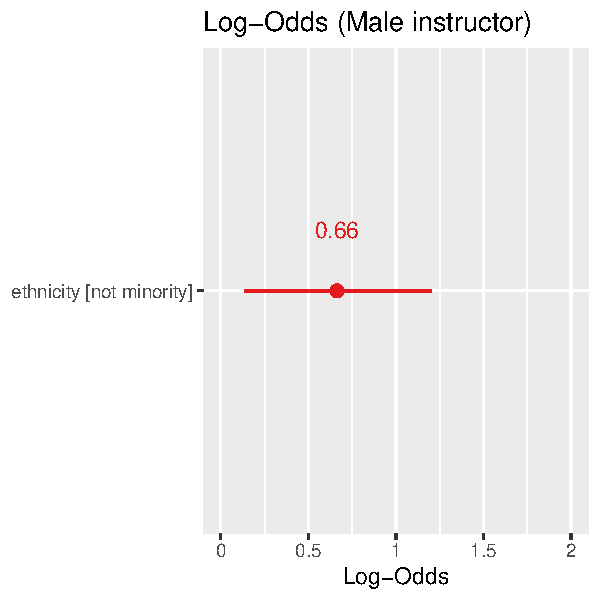
\includegraphics{index_files/figure-pdf/unnamed-chunk-47-1.pdf}

}

\caption{The log-odds for male instructors by ethnicity (not a
minority).}

\end{figure}%

\subsection{Odds}\label{odds-1}

On the \textbf{odds} scale the regression coefficients are given by

\begin{Shaded}
\begin{Highlighting}[]
\NormalTok{model.ethnic }\SpecialCharTok{\%\textgreater{}\%}
  \FunctionTok{tab\_model}\NormalTok{(}\AttributeTok{transform =} \StringTok{"exp"}\NormalTok{)}
\end{Highlighting}
\end{Shaded}

\begin{longtable}[]{@{}cccc@{}}

\caption{\label{tbl-summaries_Odds_categorical}Logistic regression with
a categorical covariate odd-scale estimates}

\tabularnewline

\toprule\noalign{}
\endhead
\bottomrule\noalign{}
\endlastfoot
~ & \multicolumn{3}{c@{}}{%
gender} \\
Predictors & Odds Ratios & CI & p \\
(Intercept) & 0.78 & 0.47~--~1.27 & 0.319 \\
ethnicity {[}not minority{]} & 1.94 & 1.14~--~3.33 & \textbf{0.015} \\
Observations & \multicolumn{3}{l@{}}{%
463} \\
R\textsuperscript{2} Tjur & \multicolumn{3}{l@{}}{%
0.013} \\

\end{longtable}

The \texttt{(Intercept)} gives us the odds of the instructor being male
given that they are in the \texttt{minority} ethnic group, that is, 0.78
(the indicator function is zero in that case).

The odds of the instructor being male given they are in the
\texttt{not\ minority} ethnic group are 1.94 times greater than the odds
if they were in the \texttt{minority} ethnic group.

Before moving on, let's break down how these values are computed. First,
the odds of the instructor being male given that they are in the
\texttt{minority} ethnic group (reference category) can be obtained as
follows:

\begin{align}
\mathrm{Odds}(\mathrm{male = 1} | \mathrm{minority} =1) &= \dfrac{p_{(minority=1)}}{1 - p_{(minority=1)}}\\
&= \exp\left(\alpha\right) \\ 
&= \exp\left(-0.25\right) \\
&= 0.78. \nonumber
\end{align}

Here,
\(p_{(minority=1)} = \mathrm{Prob}\left(\mathrm{Male}=1 | \mathrm{minority}=1\right)\).
Thus, the odds of the instructor in the \texttt{minority} group being a
male are 0.78 the odds of an instructor being a female in the same
group.

Slightly confusing right? Maybe it makes more sense to interpret this
result in terms of the \texttt{female} group,
i.e.~\(\mathrm{Odds}(\mathrm{female} = 1 | \mathrm{minority} =1)\).
However you must be aware that this is not a probability! so you can not
simply compute \(1- \mathrm{exp}(\alpha)\). To compute this correctly,
we should do as follows:

\begin{align}
\mathrm{Odds}(\mathrm{female} = 1 | \mathrm{minority} =1) &= \dfrac{P(\mathrm{female}=1 |\mathrm{minority}=1)}{P(\mathrm{male}= 1 |\mathrm{minority}=1)}\\
&= \left[\dfrac{P(\mathrm{male}=1 |\mathrm{minority}=1)}{P(\mathrm{female}= 1 |\mathrm{minority}=1)}\right]^{-1}\\
&= \left[\mathrm{Odds}(\mathrm{male}=1|\mathrm{minority}=1)\right]^{-1}\\
&= \mathrm{exp}(\alpha)^{-1} \\ &= \exp\left(-0.25\right)^{-1} = 1.28
\end{align}

Thus, the odds of the instructor in the \texttt{minority} group being a
female are 28\% higher than the odds of an instructor being a male in
the same group. However, by looking at the confidence intervals and
p-value we can see that this difference is not statistically
significant.

\begin{tcolorbox}[enhanced jigsaw, colframe=quarto-callout-warning-color-frame, toprule=.15mm, toptitle=1mm, opacitybacktitle=0.6, breakable, colback=white, opacityback=0, title={Task}, rightrule=.15mm, bottomrule=.15mm, coltitle=black, colbacktitle=quarto-callout-warning-color!10!white, leftrule=.75mm, left=2mm, arc=.35mm, bottomtitle=1mm, titlerule=0mm]

Use the \texttt{relevel} function to fit a logistic regression that
estimates the odds of the instructor being female given that they are in
the \texttt{minority} ethnic group directly.

Take hint

The reference category in your data can be changed by using the
\texttt{relevel()} function. see \texttt{?relevel} for further details.

Click here to see the solution

\begin{Shaded}
\begin{Highlighting}[]
\NormalTok{evals.ethnic }\SpecialCharTok{\%\textgreater{}\%}
  \FunctionTok{mutate}\NormalTok{(}\AttributeTok{gender =} \FunctionTok{relevel}\NormalTok{(gender,}\AttributeTok{ref =} \StringTok{"male"}\NormalTok{)) }\SpecialCharTok{\%\textgreater{}\%} 
  \FunctionTok{glm}\NormalTok{(gender }\SpecialCharTok{\textasciitilde{}}\NormalTok{ ethnicity, }\AttributeTok{data =}\NormalTok{ . ,}\AttributeTok{family =}\NormalTok{ binomial) }\SpecialCharTok{\%\textgreater{}\%} 
\NormalTok{  broom}\SpecialCharTok{::}\FunctionTok{tidy}\NormalTok{(}\AttributeTok{exponentiate =}\NormalTok{ T) }\SpecialCharTok{\%\textgreater{}\%} 
  \FunctionTok{filter}\NormalTok{(term}\SpecialCharTok{==}\StringTok{"(Intercept)"}\NormalTok{) }\SpecialCharTok{\%\textgreater{}\%}
  \FunctionTok{pull}\NormalTok{(estimate) }
\end{Highlighting}
\end{Shaded}

\begin{verbatim}
[1] 1.285714
\end{verbatim}

\end{tcolorbox}

The \texttt{ethnicity\ {[}not\ minority{]}} coefficient gives us the
odds of the instructor being male given they are \textbf{NOT} in the
minority group, i.e.,

\[
\begin{aligned}
\text{Odds}(\text{male = 1 | minority = 0}) &= \dfrac{p_{(\text{minority=0})}}{1- p_{(\text{minority=0})}}\\
&= \exp(\alpha + \beta_{\text{ethnicity}}) \\
&= \exp(-0.25 + 0.66) = 1.51
\end{aligned}
\]

Thus, non-minority-group instructors have 1.51 times higher odds of
being male compared to female.

\textbf{Comparing the odds-ratio}

Now, let's look a the \textbf{odds-ratio} of an instructor being male in
the \texttt{not\ minority} group compared to the \texttt{minority}
ethnic group, i.e.,
\(\dfrac{\text{Odds}(\text{male=1|minority=0})}{\text{Odds}(\text{male=1|minority=1})}\).

\begin{enumerate}
\def\labelenumi{\arabic{enumi}.}
\item
  First, the \textbf{odds} of an instructor being male given that they
  are in the minority ethnic group were:

  \begin{align}
  \mathrm{Odds}(\mathrm{male} = 1 | \mathrm{minority} = 1) =& 
  \dfrac{p_{(minority=1)}}{1 - p_{(minority=1)}} \\
  &= \exp\left(\alpha\right) \\ &= 0.78. \nonumber
  \end{align}
\item
  Recall that the \textbf{log-odds} of an instructor \textbf{not}
  belonging to the minority group (i.e.~\texttt{not\ minority}) being a
  male are \(\alpha +\beta_{\text{ethnicity}}\). On the odds scale this
  is:

  \begin{align}
  \mathrm{Odds}(\mathrm{male} = 1 | \mathrm{minority} = 0) =& \dfrac{p_{(\mathrm{minority} = 0)}}{1- p_{(\mathrm{minority} = 0)}}\\
  &= \mathrm{exp}( \alpha + \beta_{\text{ethnicity}}) \\
  &= 1.51
  \end{align}
\item
  Now, the odds of an instructor that is \textbf{no}t in the minority
  group being male against the odds of an instructor that comes from the
  \texttt{minority} group is given by the ratio of the odds we just
  calculated:

  \begin{align}
  \frac{\mathrm{Odds}(\mathrm{male} = 1| \mathrm{minority} = 0)}{\mathrm{Odds}(\mathrm{male} = 1| \mathrm{minority} = 1)} &= \dfrac{\frac{p_{(\mathrm{minority} = 0)}}{1- p_{(\mathrm{minority} = 0)}}}{\frac{p_{(\mathrm{minority}=1)}}{1- p_{(\mathrm{minority}=1)}}} \\
  &= \frac{\mathrm{exp}( \alpha + \beta_{\text{ethnicity}})}{\exp\left(\alpha\right)}\\ 
  &= \exp\left(\alpha + \beta_{\text{ethnicity}} - \alpha\right) \\
  &= \exp\left(\beta_{\text{ethnicity}}\right) = \exp\left(0.66 \right) \\
  &= 1.93. \nonumber 
  \end{align}
\end{enumerate}

Which is the coefficient estimate we got from the model summaries (
Table~\ref{tbl-summaries_Odds_categorical} ). This means that
instructors that are not in the minority groups are significantly 1.93
times more likely to be males compared to instructors in the minority
group.

The corresponding 95\% confidence interval of (1.14, 3.33). Again, we
can display this graphically using the \texttt{plot\_model} function
from the \texttt{sjPlot} package:

\begin{Shaded}
\begin{Highlighting}[]
\FunctionTok{plot\_model}\NormalTok{(model.ethnic,}
           \AttributeTok{transform =} \StringTok{"exp"}\NormalTok{,}
           \AttributeTok{show.values =} \ConstantTok{TRUE}\NormalTok{,}
           \AttributeTok{title =} \StringTok{"Odds (Male instructor)"}\NormalTok{,}
           \AttributeTok{show.p =} \ConstantTok{FALSE}\NormalTok{)}
\end{Highlighting}
\end{Shaded}

\begin{figure}[H]

{\centering 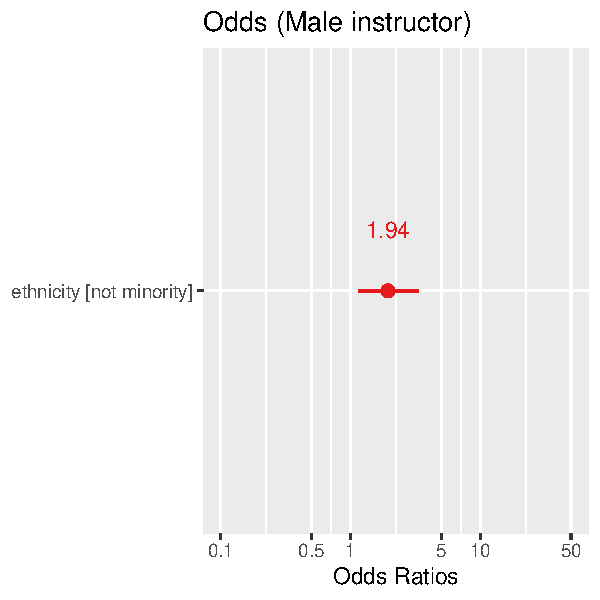
\includegraphics{index_files/figure-pdf/unnamed-chunk-51-1.pdf}

}

\caption{The odds-ratio of a male instructor given they are in the
\texttt{not\ minority} group.}

\end{figure}%

\begin{tcolorbox}[enhanced jigsaw, colframe=quarto-callout-warning-color-frame, toprule=.15mm, toptitle=1mm, opacitybacktitle=0.6, breakable, colback=white, opacityback=0, title={Task}, rightrule=.15mm, bottomrule=.15mm, coltitle=black, colbacktitle=quarto-callout-warning-color!10!white, leftrule=.75mm, left=2mm, arc=.35mm, bottomtitle=1mm, titlerule=0mm]

Calculate the odds of a \textbf{male instructor that is not} on the
minority group against the odds of a \textbf{female instructor that is}
in the minority group.

Take hint

The odds ratio of a male instructor that is not on the minority group
against the odds of a female instructor that is in the minority group
are given by:

\[
\dfrac{\text{Odds}(\text{male=1|minority=0})}{\text{Odds}(\text{female=1|minority=1})}
\]

See Solution

\[
\begin{aligned}
\dfrac{\text{Odds}(\text{male=1|minority=0})}{\text{Odds}(\text{female=1|minority=1})} &= \dfrac{\exp(\alpha+\beta_{\text{ethnicity}}) }{\exp(\alpha)^{-1}} = \dfrac{1.51}{1.28} \approx 1.18
\end{aligned}
\]

Non-minority male instructors have~\textbf{1.18 times the odds} of being
male compared to a female in the minority group.

\end{tcolorbox}

\subsection{Probabilities}\label{probabilities-1}

You can also use the model to predict the probability of having an
instructor being male for each ethnicity group.

The probabilities of an instructor being male given they are in the
\texttt{minority} and \texttt{not\ minority} groups are:

\begin{Shaded}
\begin{Highlighting}[]
\FunctionTok{plogis}\NormalTok{(}\FunctionTok{coef}\NormalTok{(model.ethnic)[}\DecValTok{1}\NormalTok{])}
\end{Highlighting}
\end{Shaded}

\begin{verbatim}
(Intercept) 
     0.4375 
\end{verbatim}

\begin{Shaded}
\begin{Highlighting}[]
\FunctionTok{plogis}\NormalTok{(}\FunctionTok{coef}\NormalTok{(model.ethnic)[}\DecValTok{1}\NormalTok{]}\SpecialCharTok{+}\FunctionTok{coef}\NormalTok{(model.ethnic)[}\DecValTok{2}\NormalTok{])}
\end{Highlighting}
\end{Shaded}

\begin{verbatim}
(Intercept) 
  0.6015038 
\end{verbatim}

Hence, the probabilities of an instructor being male given they are in
the \texttt{minority} and \texttt{not\ minority} ethnic groups are 0.437
and 0.602, respectively.

Finally, we can use the \texttt{plot\_model()} function from the
\texttt{sjPlot} package to produce the estimated probabilities by
\texttt{ethnicity} as follows:

\begin{Shaded}
\begin{Highlighting}[]
\FunctionTok{plot\_model}\NormalTok{(model.ethnic,}
           \AttributeTok{type =} \StringTok{"pred"}\NormalTok{,}
           \AttributeTok{terms =} \StringTok{"ethnicity"}\NormalTok{,}
           \AttributeTok{axis.title =} \FunctionTok{c}\NormalTok{(}\StringTok{"Ethnicity"}\NormalTok{, }
                          \StringTok{"Prob. of instructor being male"}\NormalTok{),}
           \AttributeTok{title =} \StringTok{" "}\NormalTok{)}
\end{Highlighting}
\end{Shaded}

\begin{figure}[H]

{\centering 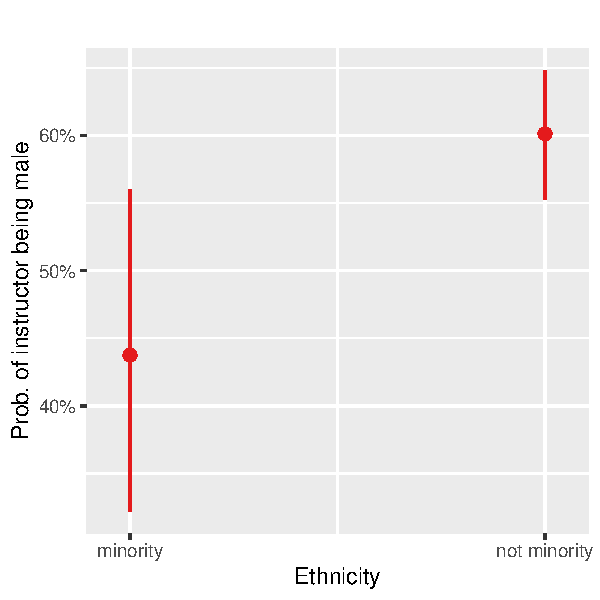
\includegraphics{index_files/figure-pdf/unnamed-chunk-54-1.pdf}

}

\caption{Probability of teaching instructor being male by ethnicity.}

\end{figure}%

\section*{The end?}\label{the-end}
\addcontentsline{toc}{section}{The end?}

Great work today! You've reached the end this session - why not take
your skills even further? Level up by tackling the
\href{about.qmd}{extra challenge tasks}.

\phantomsection\label{refs}
\begin{CSLReferences}{1}{0}
\bibitem[\citeproctext]{ref-gabry2019}
Gabry, Jonah, Daniel Simpson, Aki Vehtari, Michael Betancourt, and
Andrew Gelman. 2019. {``Visualization in Bayesian Workflow.''}
\emph{Journal of the Royal Statistical Society Series A: Statistics in
Society} 182 (2): 389--402. \url{https://doi.org/10.1111/rssa.12378}.

\bibitem[\citeproctext]{ref-gelman2006}
Gelman, Andrew, and Jennifer Hill. 2006. {``Data Analysis Using
Regression and Multilevel/Hierarchical Models,''} December.
\url{https://doi.org/10.1017/cbo9780511790942}.

\end{CSLReferences}



\end{document}
